\documentclass[10pt,conference]{IEEEtran}
\usepackage{cite}
\usepackage{url}
\usepackage{amsmath,amssymb}
\usepackage{algorithm}
\usepackage[noend]{algpseudocode}
\usepackage{booktabs}
\usepackage{multirow}
\usepackage{tikz}
\usetikzlibrary{arrows.meta,positioning,fit,backgrounds,calc,tikzmark}
\usepackage{pgfplots}
\pgfplotsset{compat=1.18}
\usepgfplotslibrary{groupplots}
\definecolor{histra}{HTML}{9ECAE1}
\pgfplotsset{
  trend/.style={scale only axis, tick label style={font=\scriptsize}, label style={font=\footnotesize},
    axis x line*=bottom, axis y line*=left, ymajorgrids, grid style={black!12}, ymin=0,
    xtick={0,1,2}, xticklabels={Easy\\200, Medium\\300, Hard\\600}, xticklabel style={align=center},
    xmin=-0.3, xmax=2.3, xlabel={Problem Difficulty}},
  lim stu/.style={black, thick, mark=*, mark size=1.7pt},
  lim ref/.style={black!45, thick, densely dashed, mark=triangle*, mark size=2.2pt, mark options={solid}},
  lim lsg/.style={black!75, thick, mark=square*, mark size=1.6pt, mark options={fill=white}},
  expg/.style={scale only axis, width=6.6cm, height=2.8cm, tick label style={font=\scriptsize}, label style={font=\footnotesize},
    xmin=-0.5, xmax=4.5, xtick={0,1,2,3,4}, xticklabels={$-$70--0, 0, 0--10, 10--30, 30--70}},
  exp count/.style={ybar, bar width=16pt, fill=black!15, draw=black!70, area legend, point meta=y, nodes near coords,
    nodes near coords style={font=\scriptsize, inner sep=1.5pt}},
  exp rate/.style={sharp plot, thick, histra!55!black, mark=*, mark size=1.8pt, point meta=y, nodes near coords,
    nodes near coords style={font=\scriptsize, inner sep=1.5pt, anchor=south, black, /pgf/number format/.cd, fixed, fixed zerofill, precision=1}},
  close/.style={scale only axis, width=6.6cm, height=3.0cm, tick label style={font=\scriptsize}, label style={font=\footnotesize},
    xmin=-0.5, xmax=3.5, xtick={0,...,3}, xticklabels={\textsc{Refactory}, \textsc{Brafar}, \textsc{LSGen}, \textsc{Histra}},
    ymin=0, ymax=100, axis x line*=bottom, ymajorgrids, grid style={black!12}},
  close bar/.style={ybar, bar width=10pt, draw=black!70, area legend, point meta=y, nodes near coords},
  close label/.style={nodes near coords style={xshift=#1, font=\scriptsize, inner sep=2.5pt, rotate=90, anchor=east,
    /pgf/number format/.cd, fixed, fixed zerofill, precision=1}},
  close kept/.style={close bar, bar shift=-5.5pt, close label=-5.5pt, fill=black!12},
  close ident/.style={close bar, bar shift=5.5pt, close label=5.5pt, fill=black!40},
  close stu/.style={sharp plot, densely dashed, black!60, no marks, forget plot},
  close dist/.style={sharp plot, black, thick, mark=*, mark size=1.7pt, point meta=y, nodes near coords,
    nodes near coords style={font=\scriptsize, inner sep=1pt, anchor=north, yshift=-2pt, fill=white, /pgf/number format/.cd, fixed, fixed zerofill, precision=1}},
}
\usepackage{listings}
\lstset{language=Python, basicstyle=\ttfamily\scriptsize, columns=fullflexible, keepspaces=true,
  numbers=left, numberstyle=\scriptsize\color{black!55}, numbersep=5pt, xleftmargin=13pt, aboveskip=2pt, belowskip=2pt,
  showstringspaces=false, escapeinside={(@}{@)}, literate={*}{{$\ast$}}1}


\begin{document}

\title{\textsc{Histra}: Guiding Program Repair for Programming Assignments with Students' Own Submission Histories}
% 학생 자신의 제출 이력으로 프로그래밍 과제 수정을 이끄는 HISTRA

\author{\IEEEauthorblockN{}
\IEEEauthorblockA{}}

\maketitle

\begin{abstract}
% 우리는 학생 자신의 제출 이력에 드러난 의도를 보존하면서 학생의 버기 제출을 수정하는 history-aware 기법인 \textsc{Histra}를 제안한다. 자동 프로그램 수정은 학생 버기 제출의 repair rate를 크게 높여 왔다. 그러나 기존 기법은 참조 프로그램, 테스트, 또는 모델이 무엇을 바꿀지 정하므로, 학생이 자신의 제출에 걸쳐 바꾸지 않고 유지해 온 코드인 ``intent skeleton''을 자주 바꾼다. 두 최신 기법의 통과 패치는 학생들이 스스로 고칠 때보다 skeleton을 2.7--3.2배 많이 바꾼다. skeleton을 보존하기는 어려운데, 이력은 수정할 영역을 거칠게만 짚고 그 영역의 올바른 코드를 담고 있지 않기 때문이다. \textsc{Histra}는 학생이 계속 고쳐 온 코드를 hole로 바꾸어 버기 제출을 스케치하고, 가장 비슷한 다른 학생들의 정답 프로그램을 검색하여 먼저 hole 안에 병합하며, hole 안의 패치가 하나도 통과하지 못할 때에만 skeleton을 바꾸고 테스트에 필요 없는 변경은 되돌린다. 14개 문제의 1,764개 trajectory에 대한 실험 결과, \textsc{Histra}는 세 최신 기법보다 4.7--76.7\% 많은 제출을 고치면서 intent skeleton을 11.7--35.2\% 적게 바꾸었고, 학생들이 자신의 수정에서 유지한 코드를 9.4--16.6\% 더 많이 유지하였다. 블라인드 평가에서 두 강사는 77.6\%의 쌍에서 이력 없이 같은 파이프라인으로 얻은 패치보다 \textsc{Histra}의 패치를 피드백으로 골랐다.
We present \textsc{Histra}, a history-aware technique that repairs buggy student submissions while preserving the intent revealed in the student's own submission history. Automated Program Repair has substantially improved the repair rate for buggy student submissions. However, existing techniques frequently change the ``intent skeleton,'' the code that a student has kept unchanged across their own submissions, because the reference programs, the tests, or a model decide which code to change. The passing patches of two state-of-the-art techniques change 2.7--3.2 times as much of the skeleton as students do in their own fixes. Preserving the skeleton is challenging because the history marks the region to repair only coarsely and contains no correct code for it. \textsc{Histra} sketches the buggy submission by turning the code that the student kept revising into holes, retrieves the accepted programs of other students most similar to it, and merges them into the holes first, changing the skeleton only when no patch confined to the holes passes and then reverting the changes that the tests do not need. Experimental results on 1,764 submission trajectories of 14 problems show that \textsc{Histra} repairs 4.7--76.7\% more submissions than three state-of-the-art techniques while changing 11.7--35.2\% less of the intent skeleton and keeping 9.4--16.6\% more of the code that students keep in their own fixes. In a blinded study, two instructors chose the patches of \textsc{Histra} as feedback over those of the same pipeline without the history in 77.6\% of the pairs.
\end{abstract}

\begin{IEEEkeywords}
Automated Program Repair, Intent Preservation, Programming Assignments, Submission History
\end{IEEEkeywords}

\section{Introduction}\label{sec:intro}

% 프로그래밍 과제를 위한 Automated Program Repair (APR)~\cite{singh2013automated, gulwani2018automated, hu2019re}은 대규모 강의의 학생들에게 피드백을 제공하는 방법으로 널리 연구되어 왔다. 기법은 버기 제출과 해당 문제의 test suite가 주어지면 모든 테스트를 통과하는 수정된 프로그램, 즉 패치를 자동으로 만들며, 덕분에 학생들은 실패한 모든 시도에 대해 피드백을 받을 수 있다~\cite{paiva2025incremental, fan2025software}. 이를 위해 기법은 제출에서 바꿀 부분을 정하고, 강사의 참조 해답, 다른 학생들의 정답 제출, 오류 모델, 또는 학습된 코드 모델로 그 부분을 대체할 코드를 합성한 뒤, 모든 테스트를 통과한 후보만 학생에게 돌려준다.
Automated Program Repair (APR) for programming assignments~\cite{singh2013automated, gulwani2018automated, hu2019re} has been widely studied as a way to provide feedback to students in large courses. Given a buggy submission and the test suite of its problem, a technique automatically produces a patch, i.e., a modified program that passes every test, so that students can receive feedback on every failed attempt~\cite{paiva2025incremental, fan2025software}. To this end, the technique determines which parts of the submission to change, synthesizes code to replace them from instructors' reference solutions, other students' correct submissions, error models, or learned code models, and returns to the student only a candidate that passes every test.

% 학생 프로그램의 수정에는 두 가지 열린 문제가 있다. 하나는 초보자의 프로그램에서 잘못된 부분을 찾는 것이고, 다른 하나는 방대한 후보 공간에서 그 부분에 들어갈 올바른 코드를 합성하는 것이다. 기존 기법들은 고칠 부분을 찾는 방식에 따라 세 가지로 나뉜다. alignment-based 기법은 버기 제출을 다른 학생들의 정답 제출이나 강사의 해답과 정렬하여 서로 갈라지는 부분을 고치고~\cite{gulwani2018automated, wang2018search, hu2019re, ahmed2022verifix, choi2021automated, choi2025automated}, localization-based 기법은 실패한 테스트로 결함 위치를 추정하여 그 부분을 고친다~\cite{xie2024brafar, orvalho2025counterexample, dai2025less}. knowledge-based 기법은 강사가 작성한 오류 모델, 다른 학생들의 수정에서 학습한 변환, 또는 Large Language Model(LLM)처럼 흔한 실수와 그 수정에 대한 지식으로 고칠 부분과 코드를 함께 정한다~\cite{singh2013automated, rolim2017learning, heo2023referent, zhang2024pydex, zhao2024peer, dai2026learner}. 이 기법들은 학생 제출의 repair rate를 크게 높여 왔다.
Repairing student programs poses two open problems: locating the faulty parts of a novice's program, and synthesizing correct code for them in a vast space of candidates. Existing techniques fall into three groups by how they locate the parts to repair. Alignment-based techniques align the submission with other students' correct submissions or an instructor's solution and repair the parts where the two diverge~\cite{gulwani2018automated, wang2018search, hu2019re, ahmed2022verifix, choi2021automated, choi2025automated}, and localization-based techniques localize faults with the failing tests and repair the suspected parts~\cite{xie2024brafar, orvalho2025counterexample, dai2025less}. Knowledge-based techniques decide both the parts and the code with knowledge of common mistakes and their fixes, such as an instructor-written error model, transformations learned from the fixes of other students, or a Large Language Model (LLM)~\cite{singh2013automated, rolim2017learning, heo2023referent, zhang2024pydex, zhao2024peer, dai2026learner}. These techniques have substantially raised the repair rate for student submissions.

% 그러나 기존 기법은 학생이 프로그램의 어느 부분을 확정했는지 알지 못한다. 패치가 무엇을 남길지는 테스트나 다른 학생의 해답이 정하며, 학생 프로그램에 가까운 패치를 선호하는 기법도 모든 부분을 똑같이 다룬다. 피드백은 학습자 자신의 작업에 구체적일 때 효과적이므로~\cite{hattie2007power, shute2008focus}, 교육용 수정 연구는 학생 프로그램과의 가까움을 패치의 품질 기준으로 삼는다~\cite{koutcheme2023evaluating, koutcheme2025direct}. 다시 작성된 패치는 정답을 드러낼 뿐 시도의 무엇이 틀렸는지는 감추며, 자동 생성된 수정만으로는 초보자에게 도움이 적다~\cite{yi2017feasibility}. 본 연구에서는 버기 제출 중 학생이 연속된 버기 제출에 걸쳐 바꾸지 않은 부분을 \emph{intent skeleton}으로, 패치가 그중 바꾼 비율을 \emph{skeleton loss}로 정의한다. 학생들은 스스로 정답에 이를 때 절반 이상(61.3\%)이 intent skeleton을 전혀 바꾸지 않았지만, 두 최신 기법~\cite{hu2019re, dai2026learner}의 통과 패치는 70.0\%와 73.7\%가 skeleton을 바꾸었고 바꾼 양도 학생의 2.7--3.2배였다(Section~\ref{sec:prelim-limit}). 도움을 받는 학생의 이력 없이는, 이 기법들은 학생 자신의 시도에 대한 피드백 대신 다른 사람의 해답을 따른 프로그램을 줄 수 있다.
However, existing techniques do not know which parts of a program the student has settled on. Which code a patch keeps is decided by the tests or by other students' solutions, and even techniques that prefer patches close to the student's program treat every part of it alike. Because feedback is more effective when it is specific to the learner's own work~\cite{hattie2007power, shute2008focus}, work on educational repair treats closeness to the student's program as a quality criterion~\cite{koutcheme2023evaluating, koutcheme2025direct}. A rewritten patch reveals a correct answer but hides what was wrong with the attempt, and generated repairs alone help novices little~\cite{yi2017feasibility}. In this work, we define the \emph{intent skeleton} of a buggy submission as the part that the student kept across their successive buggy submissions, and the \emph{skeleton loss} of a patch as the fraction of the intent skeleton that the patch changes. More than half (61.3\%) of the students' own fixes leave the intent skeleton entirely unchanged, whereas 70.0\% and 73.7\% of the passing patches of two state-of-the-art techniques~\cite{hu2019re, dai2026learner} change it, and they change 2.7 to 3.2 times as much of it as the students do (Section~\ref{sec:prelim-limit}). Without the history of the student being helped, these techniques may give the student a program shaped by someone else's solution rather than feedback on their own attempt.

% 본 논문에서는 학생 자신의 제출 이력에 드러난 의도를 보존하면서 버기 제출을 수정하는 history-aware 기법인 \textsc{Histra}를 제안한다. 핵심 아이디어는 학생의 버기 제출들이 이미 그 학생의 의도를 기록하고 있다는 것이다. 모든 수정에서 살아남은 코드는 학생이 확정한 부분일 가능성이 높고, 계속 바뀌는 코드는 학생이 막혀 있는 부분일 가능성이 높다. 다만 이 단서는 거칠기 때문에(Section~\ref{sec:prelim-limit}), \textsc{Histra}는 후자에 수정을 집중하되 이를 제약이 아닌 선호로 쓴다. Sketch 단계에서 \textsc{Histra}는 tree edit distance로 마지막 버기 제출을 이전 제출들과 정렬하여, 모든 제출에 걸쳐 유지된 코드를 intent skeleton으로 표시하고 나머지를 hole로 바꾼다. 결함 위치 추정(FL)이나 오류 모델에서 얻는 기존 기법의 hole과 달리, 이 hole은 학생 자신이 고쳐 온 곳을 가리킨다. Search 단계에서는 버기 제출과 가장 비슷한 다른 학생들의 참조 프로그램을 검색한다. Repair 단계에서는 이를 먼저 hole 안에 병합하고, 그런 패치가 통과하지 못할 때에만 skeleton을 더 많이 유지하는 후보부터 skeleton도 바꾸는 후보를 검증하며, 테스트에 필요 없는 변경은 되돌린다. 그 결과 패치는 학생의 intent skeleton을 유지하는 경향이 있다.
In this paper, we present \textsc{Histra}, a history-aware technique that repairs buggy submissions while preserving the intent revealed in the student's own submission history. Our key idea is that a student's buggy submissions already record the student's intent: code that survives every revision is likely what the student has settled on, whereas code that keeps changing is likely where the student is stuck. Because this signal is coarse (Section~\ref{sec:prelim-limit}), \textsc{Histra} focuses the repair on the latter but treats it as a preference rather than a constraint. In the Sketch stage, \textsc{Histra} aligns the latest buggy submission with the earlier ones using tree edit distance, marks the code kept across all of them as the intent skeleton, and turns the rest into holes. Unlike the holes of existing techniques, which come from Fault Localization (FL) or an error model, these holes mark the code that the student has kept revising. In the Search stage, it retrieves the reference programs of other students most similar to the buggy submission. In the Repair stage, it first merges them only into the holes, validates the candidates that also change the skeleton only when no such patch passes, starting from those that keep more of it, and reverts the changes that the tests do not need. As a result, the patches tend to keep the student's intent skeleton.

% 실험 결과는 \textsc{Histra}가 가장 많은 제출을 고치면서도 학생의 intent skeleton을 가장 적게 바꿈을 보여 준다. 우리는 Project CodeNet~\cite{puri2021codenet}의 AtCoder 14개 문제에서 수집한 1,764개의 submission trajectory로 \textsc{Histra}를 세 계열의 최신 기법인 \textsc{Refactory}~\cite{hu2019re}, \textsc{Brafar}~\cite{xie2024brafar}, \textsc{LSGen}~\cite{dai2026learner}과 비교하였다. \textsc{Histra}는 버기 제출의 96.5\%를 고쳐 baseline들보다 4.7--76.7\% 많이 고쳤다. 통과 패치는 평균적으로 skeleton의 18.7\%만 바꾸어 baseline들보다 11.7--35.2\% 적게 바꾸었고, skeleton을 전혀 바꾸지 않은 패치도 42.0--149.7\% 많았다. 이력을 빼거나 이력 대신 FL로 hole을 정하면 skeleton loss가 각각 32.1\%와 11.6\% 늘었다. 모든 기법이 고친 trajectory에서 \textsc{Histra}의 패치는 학생들이 자신의 수정에서 유지한 코드를 baseline들보다 9.4--16.6\% 더 많이 유지하였다. 두 강사도 이력 없이 같은 파이프라인으로 만든 패치보다 \textsc{Histra}의 패치를 피드백으로 선호하였다(Section~\ref{sec:rq-expert}).
Experimental results demonstrate that \textsc{Histra} repairs the most submissions while changing the least of the student's intent skeleton. We evaluated \textsc{Histra} on 1,764 submission trajectories of 14 AtCoder problems from Project CodeNet~\cite{puri2021codenet} against state-of-the-art techniques of the three groups: \textsc{Refactory}~\cite{hu2019re}, \textsc{Brafar}~\cite{xie2024brafar}, and \textsc{LSGen}~\cite{dai2026learner}. \textsc{Histra} fixed 96.5\% of the buggy submissions, 4.7--76.7\% more than the baselines. Its passing patches changed only 18.7\% of the skeleton on average, 11.7--35.2\% less than those of the baselines, and left the skeleton entirely unchanged 42.0--149.7\% more often. Without the history and with holes from FL instead of the history, the skeleton loss increased by 32.1\% and 11.6\%, respectively. On the trajectories that all techniques fixed, the patches of \textsc{Histra} kept 9.4--16.6\% more of the code that the students kept in their own fixes than those of the baselines. Two instructors also preferred the patches of \textsc{Histra} as feedback to those of the same pipeline without the history (Section~\ref{sec:rq-expert}).

% \textbf{기여.} 본 논문의 기여는 다음과 같다:
% \begin{itemize}
%   \item \textbf{관찰:} 최신 기법의 패치가 학생들이 스스로 고칠 때보다 intent skeleton을 훨씬 많이 바꿈을 보이고, 이를 통해 학생 자신의 제출 이력에 기반한 수정의 필요성을 제시한다.
%   \item \textbf{새로운 기법:} 프로그래밍 과제를 위한 intent-preserving repair 기법인 \textsc{Histra}를 제안한다. 핵심 기술적 기여는 FL이나 오류 모델이 아닌 학생 자신의 제출 이력에서 hole을 얻고, 이를 제약이 아닌 선호로 쓰는 수정 알고리즘이다.
%   \item \textbf{평가:} 1,764개 trajectory에서 \textsc{Histra}를 최신 기법 및 대조군들과 비교하여 그 효과를 입증한다. \textsc{Histra}는 가장 많은 제출을 고치면서도 intent skeleton을 가장 적게 바꾸었고, 강사들은 그 패치를 피드백으로 선호하였다.
% \end{itemize}
\textbf{Contributions.} We summarize our contributions below:
\begin{itemize}
  \item \textbf{Observation:} We show that the patches of state-of-the-art techniques change much more of the intent skeleton than students do in their own fixes, motivating the need for repair that conditions on the student's own submission history.
  \item \textbf{New technique:} We present \textsc{Histra}, an intent-preserving repair technique for programming assignments. Our core technical contribution is a repair algorithm that derives the holes from the student's own submission history rather than from FL or an error model and uses them as a preference rather than a constraint.
  \item \textbf{Evaluation:} We demonstrate the effectiveness of \textsc{Histra} by comparing it with state-of-the-art techniques and controls on 1,764 trajectories: \textsc{Histra} repaired the most submissions while changing the least of the intent skeleton, and instructors preferred its patches as feedback.
\end{itemize}

\section{Preliminaries}\label{sec:prelim}

\subsection{Automated Program Repair for Programming Assignments}\label{sec:prelim-repair}

% 프로그래밍 과제를 위한 APR의 주된 목표는 버기 제출을 해당 문제의 test suite를 통과하는 프로그램으로 바꾸는 것이며, 흔히 \emph{참조 프로그램}, 즉 같은 문제에 대한 동료 학생들의 정답 프로그램을 이용한다. 우리는 한 학생의 \emph{submission trajectory}를 학생의 버기 제출을 시간 순으로 나열하고 첫 정답 제출을 덧붙인 수열 $\langle P_1, \ldots, P_n, P_{\mathit{ac}} \rangle$로 정의한다. $P_{\mathit{ac}}$는 평가의 기준으로만 쓰이며 기법에는 주어지지 않는다. 수정할 마지막 버기 제출 $b = P_n$을 \emph{버기 프로그램}, 그 이전의 제출 $H = \langle P_1, \ldots, P_{n-1} \rangle$을 학생의 \emph{이력 프로그램}이라 부른다.
The main aim of APR for programming assignments is to turn a buggy submission into a program that passes the test suite of its problem, often by using \emph{reference programs}, i.e., accepted programs that peer students wrote for the same problem. We define the \emph{submission trajectory} of a student as a sequence $\langle P_1, \ldots, P_n, P_{\mathit{ac}} \rangle$ of the student's buggy submissions in chronological order followed by their first accepted submission $P_{\mathit{ac}}$, which serves only as ground truth for evaluation and is never given to a technique. We call the latest buggy submission $b = P_n$, which is to be repaired, the \emph{buggy program}, and the earlier ones, $H = \langle P_1, \ldots, P_{n-1} \rangle$, the student's \emph{history programs}.

\begin{algorithm}[h]
\caption{APR for Programming Assignments}\label{alg:generic}
\footnotesize
\begin{algorithmic}[1]
\item[\textbf{Input:}] Buggy program ($b$), Test suite ($T$), Reference programs ($R$).
\item[\textbf{Output:}] Fixed program ($f$), or $\bot$ if none is found
\Procedure{APR}{$b, T, R$}
  \For{$r \in \mathsf{Rank}(R, b)$}
    \State $b^{\square} \gets \mathsf{Sketch}(b, T, r)$ \Comment{parts of $b$ to repair as holes}
    \State $f \gets \mathsf{Merge}(b^{\square}, r)$ \Comment{fill the holes with the code of $r$}
    \If{$\mathsf{Validate}(f, T)$}
      \State \Return $f$
    \EndIf
  \EndFor
  \State \Return $\bot$
\EndProcedure
\end{algorithmic}
\end{algorithm}

% Algorithm~\ref{alg:generic}은 기존 기법들~\cite{gulwani2018automated, wang2018search, hu2019re}의 방식에 따라 프로그래밍 과제를 위한 일반적인 수정 알고리즘을 기술한다. 이 알고리즘은 버기 프로그램($b$), test suite($T$), 참조 프로그램 집합($R$)을 입력으로 받아, 모든 테스트를 통과하는 수정된 프로그램($f$)을 반환한다. 2번째 줄에서 알고리즘은 $R$의 프로그램들에 $b$와의 유사도로 순위를 매기고, 순위가 높은 프로그램 $r$부터 차례로 수정을 시도한다. 3번째 줄에서 함수 $\mathsf{Sketch}$는 $b$에서 수정할 부분을 hole로 표시한 \emph{스케치}~\cite{solar2006combinatorial} $b^{\square}$를 반환한다. 4번째 줄에서 함수 $\mathsf{Merge}$는 $b^{\square}$를 $r$과 정렬하여 hole을 $r$의 코드로 채운다. 병합된 프로그램이 $T$의 모든 테스트를 통과하면 즉시 그 프로그램을 $f$로 반환하고(5--6번째 줄), 어떤 참조 프로그램으로도 그러한 프로그램을 얻지 못하면 $\bot$을 반환한다(7번째 줄).
Algorithm~\ref{alg:generic} describes a generic repair algorithm for programming assignments in the style of existing techniques~\cite{gulwani2018automated, wang2018search, hu2019re}. It takes the buggy program ($b$), a test suite ($T$), and a set of reference programs ($R$) as input, and returns a fixed program ($f$) that passes every test. At line~2, the algorithm ranks the programs in $R$ by their similarity to $b$ and tries them in turn, starting from the top-ranked program $r$. At line~3, the function $\mathsf{Sketch}$ returns a \emph{sketch}~\cite{solar2006combinatorial} $b^{\square}$, i.e., $b$ with the parts to repair marked as holes. At line~4, the function $\mathsf{Merge}$ aligns $b^{\square}$ with $r$ and fills the holes with the code of $r$. As soon as the merged program passes every test in $T$, it returns that program as $f$ (lines~5--6); if no reference program yields such a program, it returns $\bot$ (line~7).

% 기존 기법들은 3번째 줄에서 $b$의 어느 부분을 고칠지 정하는 방식에 따라 세 가지로 나뉜다. alignment-based 기법은 $r$과의 정렬 한 번으로 3--4번째 줄을 수행하여 $b$가 $r$과 갈라지는 부분을 고친다. \textsc{Clara}~\cite{gulwani2018automated}와 \textsc{Sarfgen}~\cite{wang2018search}은 제어 흐름이 같은 참조 프로그램이 필요하고, \textsc{Refactory}~\cite{hu2019re}는 참조 프로그램을 리팩터링하되 그래도 맞지 않으면 학생이 무엇을 확정했는지와 무관하게 $b$의 제어 흐름을 변형하며, \textsc{Mentored}~\cite{choi2025automated}는 다른 학생들의 프로그램을 조합해 새로운 구조를 만든다. localization-based 기법은 $T$의 실패한 테스트로 결함 위치를 추정한다. \textsc{Brafar}~\cite{xie2024brafar}는 $b$와 $r$의 실행을 블록 단위로 비교하고, \textsc{Cegis}~\cite{orvalho2025counterexample}는 MaxSAT 기반 fault localization으로 hole을 만들어 LLM이 채우게 한다. knowledge-based 기법은 3--4번째 줄(흔히 2번째 줄도)을 오류 모델~\cite{singh2013automated}, 학습된 변환~\cite{rolim2017learning}, 또는 LLM~\cite{heo2023referent, zhang2024pydex, zhao2024peer, dai2026learner}으로 대체한다. 이들 중 일부는 후보 중 가장 작은 패치나 $b$에 가장 가까운 패치를 고른다~\cite{gulwani2018automated, wang2018search, ahmed2022verifix, d2016qlose, zhang2024pydex}. 어느 경우든 $b$의 어느 부분을 고칠지는 참조 프로그램, 테스트, 또는 지식이 정하며, 학생의 이력은 쓰이지 않는다.
Existing techniques fall into three groups by how they decide, at line~3, which parts of $b$ to repair. Alignment-based techniques perform lines~3--4 through a single alignment with $r$ and repair the parts where $b$ diverges from $r$: \textsc{Clara}~\cite{gulwani2018automated} and \textsc{Sarfgen}~\cite{wang2018search} require a reference program with the same control flow; \textsc{Refactory}~\cite{hu2019re} refactors the reference programs and, failing that, mutates the control flow of $b$ without regard to which parts the student has settled on; and \textsc{Mentored}~\cite{choi2025automated} combines the programs of other students into new structures. Localization-based techniques localize faults with the failing tests in $T$: \textsc{Brafar}~\cite{xie2024brafar} compares the executions of $b$ and $r$ block by block, and \textsc{Cegis}~\cite{orvalho2025counterexample} derives holes from MaxSAT-based fault localization and lets an LLM fill them. Knowledge-based techniques replace lines~3--4, and often line~2, with an error model~\cite{singh2013automated}, learned transformations~\cite{rolim2017learning}, or an LLM~\cite{heo2023referent, zhang2024pydex, zhao2024peer, dai2026learner}. Some of these techniques select the smallest patch or the patch closest to $b$ among the candidates~\cite{gulwani2018automated, wang2018search, ahmed2022verifix, d2016qlose, zhang2024pydex}. In all cases, which parts of $b$ to repair is decided by the reference programs, the tests, or the knowledge; the student's history is not used.

\subsection{Limitation of History-Agnostic Repair}\label{sec:prelim-limit}

% 우리의 핵심 관찰은 학생의 이력 없이 만들어진 패치가 학생이 유지해 온 코드를 자주 덮어쓴다는 것이다. 이를 정량화하기 위해 Section~\ref{sec:intro}에서 소개한 intent skeleton을 형식화한다. $b$와 이력 프로그램 $H$가 주어지면, 먼저 표면적 차이를 없애기 위해 모든 제출을 정규화하고(Section~\ref{sec:sketch}), 각 $P_i \in H$에 대해 tree edit distance~\cite{bille2005survey, pawlik2016tree}를 이용해 정규화된 Abstract Syntax Tree(AST) $\hat{P}_i$와 $\hat{b}$ 사이의 minimum-cost edit mapping $M_i$를 계산한다. 모든 $i < n$에 대해 $M_i$가 $\hat{b}$의 노드 $w$를 같은 타입의 노드에 대응시키면, $w$를 \emph{stable} 노드라고 부른다. 엄밀히 말해, intent skeleton은 자신과 모든 문장 및 식 조상이 stable한 $\hat{b}$의 문장 및 식 노드의 집합이다:
% \[ \mathit{Skel}(\hat{b}) = \{\, v \in \hat{U} \mid \forall w \in \mathit{anc}^{*}(v) \cap \hat{U}.\ \mathit{stable}(w) \,\} \]
% 여기서 $\hat{U}$는 $\hat{b}$의 문장 및 식 노드이고, $\mathit{anc}^{*}(v)$는 $v$와 그 조상들을 나타낸다. Section~\ref{sec:sketch}는 이 집합을 학생의 원래 코드 위로 옮기며, 그 결과를 $\mathit{Skel}(b)$로 쓴다. 수정된 프로그램 $f$가 skeleton을 얼마나 바꾸는지는 주된 지표인 \emph{skeleton loss}, 즉 $b$와 $f$ 사이의 minimum-cost edit mapping에서 $f$의 동일한 노드에 대응되지 않는 $\mathit{Skel}(b)$ 노드의 비율로 잰다. 두 노드는 타입과 식별자·상수·연산자가 같을 때 동일하므로, stability와 달리 skeleton 안의 상수나 연산자를 바꾸어도 손실로 센다. skeleton loss가 0인 패치를 \emph{intact patch}라 부른다.
Our key observation is that patches produced without the student's history frequently overwrite the code that the student has kept. To quantify this, we formalize the intent skeleton introduced in Section~\ref{sec:intro}. Given $b$ and the history programs $H$, we first normalize all submissions to remove surface variations (Section~\ref{sec:sketch}) and compute, for each $P_i \in H$, the minimum-cost edit mapping $M_i$ between the normalized Abstract Syntax Trees (ASTs) $\hat{P}_i$ and $\hat{b}$ using tree edit distance~\cite{bille2005survey, pawlik2016tree}. We call a node $w$ of $\hat{b}$ \emph{stable} if, for every $i < n$, $M_i$ maps $w$ to a node of the same type. Formally, the intent skeleton is the set of statement and expression nodes of $\hat{b}$ that, together with all their statement and expression ancestors, are stable:
\[ \mathit{Skel}(\hat{b}) = \{\, v \in \hat{U} \mid \forall w \in \mathit{anc}^{*}(v) \cap \hat{U}.\ \mathit{stable}(w) \,\} \]
where $\hat{U}$ denotes the statement and expression nodes of $\hat{b}$ and $\mathit{anc}^{*}(v)$ denotes $v$ and its ancestors. Section~\ref{sec:sketch} maps this set onto the student's original code; we write $\mathit{Skel}(b)$ for the result. We measure how much of the skeleton a fixed program $f$ changes by its \emph{skeleton loss}, our main metric: the fraction of the nodes in $\mathit{Skel}(b)$ that are not mapped to an identical node of $f$ under the minimum-cost edit mapping between $b$ and $f$, where two nodes are identical if they have the same type and the same identifier, constant, or operator. Unlike stability, the loss thus also counts a changed constant or operator in the skeleton. We call a patch with no skeleton loss an \emph{intact patch}.

\begin{figure}[h]
\centering
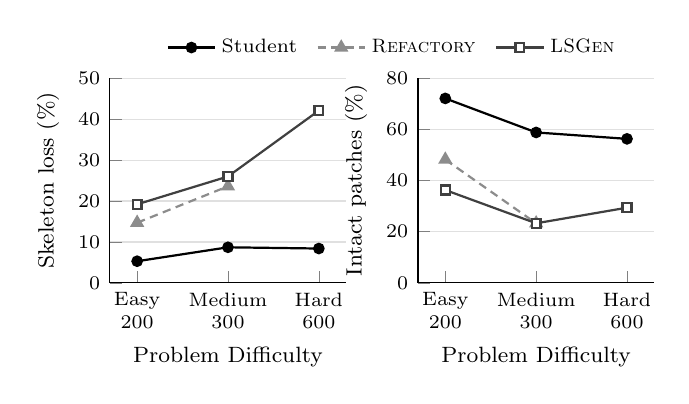
\begin{tikzpicture}
\begin{groupplot}[group style={group size=2 by 1, horizontal sep=26pt}, trend, width=3.0cm, height=2.6cm]
\nextgroupplot[ymax=50, ytick={0,10,20,30,40,50}, ylabel={Skeleton loss (\%)},
  legend entries={Student, \textsc{Refactory}, \textsc{LSGen}},
  legend style={at={(1.2,1.05)}, anchor=south, legend columns=-1, draw=none, font=\scriptsize,
    /tikz/every even column/.append style={column sep=5pt}}]
% rows:figlimitloss
\addplot[lim stu] coordinates {(0,5.3) (1,8.7) (2,8.4)};
\addplot[lim ref] coordinates {(0,14.7) (1,23.6)};
\addplot[lim lsg] coordinates {(0,19.2) (1,26.0) (2,42.1)};
% end rows
\nextgroupplot[ymax=80, ytick={0,20,40,60,80}, ylabel={Intact patches (\%)}]
% rows:figlimitintact
\addplot[lim stu] coordinates {(0,72.1) (1,58.8) (2,56.3)};
\addplot[lim ref] coordinates {(0,48.2) (1,23.3)};
\addplot[lim lsg] coordinates {(0,36.3) (1,23.3) (2,29.4)};
% end rows
\end{groupplot}
\end{tikzpicture}
\caption{Skeleton loss and intact patches by problem difficulty}
\label{fig:limit}
\end{figure}

% Figure~\ref{fig:limit}은 우리 벤치마크(Section~\ref{sec:settings})에서 학생 자신의 정답 제출과 두 최신 기법 \textsc{Refactory}~\cite{hu2019re}, \textsc{LSGen}~\cite{dai2026learner}의 통과 패치가 intent skeleton을 얼마나 바꾸었는지를, AtCoder 배점에 따른 난이도(쉬움 200점, 보통 300점, 어려움 600점)별로 보여 준다(왼쪽: 평균 skeleton loss, 오른쪽: intact 패치 비율). 학생 자신의 정답 제출은 61.3\%가 intact 패치였지만, \textsc{Refactory}와 \textsc{LSGen}의 통과 패치는 30.0\%와 26.3\%뿐이었고, 평균적으로 skeleton의 21.2\%와 25.3\%를 바꾸어 학생(8.0\%)의 2.7배와 3.2배에 이르렀다. 학생들은 난이도와 무관하게 skeleton을 비슷하게 바꾸었지만(5.3--8.7\%), 기법은 어려운 문제일수록 더 많이 바꾸었다(\textsc{Refactory} 14.7\%, 23.6\%; \textsc{LSGen} 19.2\%, 26.0\%, 42.1\%; \textsc{Refactory}는 어려운 문제에서 통과 패치를 만들지 못하였다). 또한 학생들은 스스로 고칠 때 skeleton 노드의 9.8\%만 바꾼 반면 나머지 노드는 18.8\%를 바꾸어, intent skeleton이 학생들이 유지하기로 한 코드를 대체로 반영함을 보여 준다.
Figure~\ref{fig:limit} shows how much of the intent skeleton the students' own accepted submissions and the passing patches of two state-of-the-art techniques, \textsc{Refactory}~\cite{hu2019re} and \textsc{LSGen}~\cite{dai2026learner}, changed on our benchmark (Section~\ref{sec:settings}), by difficulty according to the point values of the problems in the AtCoder contests (easy: 200, medium: 300, and hard: 600 points; left: mean skeleton loss; right: share of intact patches). When the students fixed their own programs, 61.3\% of their accepted submissions were intact patches, whereas only 30.0\% and 26.3\% of the passing patches of \textsc{Refactory} and \textsc{LSGen} were, and these patches changed 21.2\% and 25.3\% of the skeleton on average, 2.7 and 3.2 times as much as the students did (8.0\%). The students changed a similar share of the skeleton regardless of difficulty (5.3--8.7\%), but the techniques changed more of it on harder problems (\textsc{Refactory} 14.7\% and 23.6\%; \textsc{LSGen} 19.2\%, 26.0\%, and 42.1\%; \textsc{Refactory} produced no passing patch on the hard problem). Moreover, in their own fixes the students changed only 9.8\% of the skeleton nodes but 18.8\% of the other nodes, which shows that the skeleton largely reflects code that the students chose to keep.

% 수정을 최소화하는 것만으로는 이 문제를 풀 수 없다. 두 기법은 이미 최소 수정을 지향한다. \textsc{Refactory}는 최소한의 수정을 합성하고~\cite{hu2019re}, \textsc{LSGen}은 원래의 구조와 논리를 보존하도록 최소한으로 고치라고 모델에 지시한다~\cite{dai2026learner}. 그런데도 두 기법의 통과 패치는 skeleton의 21.2\%와 25.3\%를 바꾸었다. 최소 수정은 프로그램의 모든 부분을 똑같이 다루므로, 학생이 확정한 코드와 계속 고쳐 온 코드를 구별하지 못하기 때문이다.
Minimizing the repair alone does not solve this problem. Both techniques already aim at minimal repairs: \textsc{Refactory} synthesizes minimal repairs~\cite{hu2019re}, and \textsc{LSGen} instructs the model to make minimal changes that preserve the original structure and logic~\cite{dai2026learner}. Nevertheless, their passing patches changed 21.2\% and 25.3\% of the skeleton, because minimal repair treats every part of the program alike and thus cannot tell the code that the student has settled on from the code that the student kept revising.

% 이러한 한계는 우리의 접근법의 동기가 된다. 우리의 목표는 참조 프로그램만을 수정 재료로 사용하여, Algorithm~\ref{alg:generic}의 스케치를 학생의 이력 $H$로부터 만들어, $b$를 $T$를 통과하면서 $\mathit{Skel}(b)$를 최대한 유지하는 프로그램 $f$로 고치는 것이다. 그러나 이력은 수정할 위치를 거칠게만 짚는다. 학생 자신의 수정은 skeleton 밖 코드의 18.8\%만 바꾸고, 수정이 바꾼 노드 중 skeleton 밖에 있는 것도 64.4\%뿐이다. 더욱이 이력에는 고칠 부분의 올바른 코드가 없으므로, 수정 재료는 식별자와 구조가 학생과 다른 참조 프로그램에서 가져와야 한다. 따라서 본 연구는 두 가지 핵심 난제를 다룬다: (1) 이력이 결함 위치를 거칠게만 짚는 버기 프로그램을 수정하는 것, 그리고 (2) 수정할 부분을 참조 프로그램의 코드로 채우면서 나머지 부분에서는 학생의 식별자와 구조를 유지하는 것.
These limitations motivate our approach. Our goal is to repair $b$, using only the reference programs as repair material, into a fixed program $f$ that passes $T$ and retains as much of $\mathit{Skel}(b)$ as possible, by deriving the sketch of Algorithm~\ref{alg:generic} from the student's history $H$. However, the history marks where to repair only coarsely: the student's own fix changes only 18.8\% of the code outside the skeleton, and only 64.4\% of the nodes that the fix changes lie outside the skeleton. Moreover, the history contains no correct code for the parts to be repaired, so the repair material must come from the reference programs, whose identifiers and structure differ from the student's. Our work thus tackles two key challenges: (1) repairing a buggy program whose history localizes the fault only coarsely, and (2) filling the parts to be repaired with code from the reference programs while keeping the student's identifiers and structure elsewhere.

\section{Our Approach}\label{sec:approach}

\begin{figure}[h]
\centering
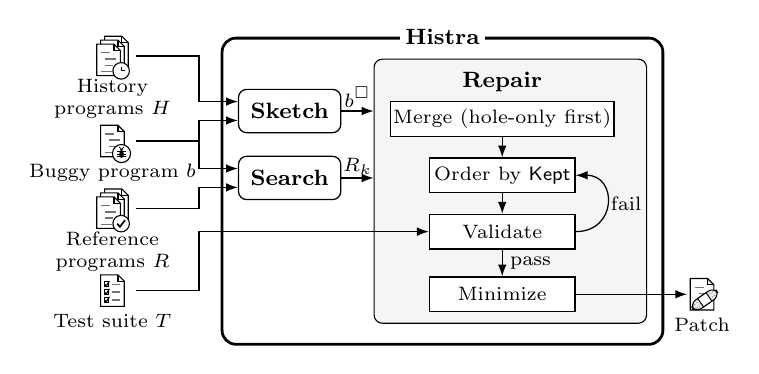
\begin{tikzpicture}[font=\scriptsize, >={Latex[length=1.5mm,width=1.1mm]}, line width=0.45pt,
  stage/.style={draw, rounded corners=3pt, minimum width=13mm, minimum height=5.5mm, align=center, font=\footnotesize\bfseries, fill=white},
  sub/.style={draw, minimum width=18.5mm, minimum height=4.4mm, inner sep=1pt, align=center, fill=white},
  io/.style={align=left, inner sep=1pt},
  lbl/.style={font=\scriptsize, inner sep=1.2pt},
  icpage/.pic={\draw[fill=white, line width=0.4pt] (-1.5mm,-2mm) -- (-1.5mm,2mm) -- (0.7mm,2mm) -- (1.5mm,1.2mm) -- (1.5mm,-2mm) -- cycle;
             \draw[line width=0.4pt] (0.7mm,2mm) -- (0.7mm,1.2mm) -- (1.5mm,1.2mm);},
  iccode/.pic={\pic{icpage};
             \foreach \y/\u/\v in {0.9/-0.9/0.2, 0.1/-0.4/0.9, -0.7/-0.4/0.6, -1.5/-0.9/0.4}
               \draw[line width=0.5pt, black!55] (\u mm,\y mm) -- (\v mm,\y mm);},
  icstack/.pic={\pic at (1mm,1mm) {icpage}; \pic at (0.5mm,0.5mm) {icpage}; \pic{iccode};},
  icbadge/.pic={\draw[fill=white, line width=0.4pt] (0,0) circle (1.05mm);},
  ichistory/.pic={\pic at (-0.5mm,-0.5mm) {icstack};
                \pic at (1.1mm,-1.9mm) {icbadge};
                \draw[line width=0.4pt] (1.1mm,-1.35mm) -- (1.1mm,-1.9mm) -- (1.55mm,-1.9mm);},
  iccorrect/.pic={\pic at (-0.5mm,-0.5mm) {icstack};
                \pic at (1.1mm,-1.9mm) {icbadge};
                \draw[line width=0.6pt] (0.6mm,-1.9mm) -- (0.95mm,-2.3mm) -- (1.6mm,-1.45mm);},
  ictests/.pic={\pic{icpage};
              \foreach \y in {0.8,-0.2,-1.2} {
                \draw[line width=0.35pt] (-1.05mm,\y mm-0.3mm) rectangle (-0.45mm,\y mm+0.3mm);
                \draw[line width=0.45pt] (-1.0mm,\y mm) -- (-0.8mm,\y mm-0.25mm) -- (-0.4mm,\y mm+0.4mm);
                \draw[line width=0.5pt, black!55] (-0.1mm,\y mm) -- (1.0mm,\y mm);}},
  icbandage/.pic={\begin{scope}[rotate=35]
                \draw[fill=black!8, line width=0.4pt, rounded corners=0.9mm] (-2.6mm,-0.9mm) rectangle (2.6mm,0.9mm);
                \draw[fill=white, line width=0.35pt] (-0.9mm,-0.9mm) rectangle (0.9mm,0.9mm);
                \foreach \x in {-1.9,-1.4,1.4,1.9} \foreach \y in {-0.35,0.35} \fill[black!45] (\x mm,\y mm) circle (0.13mm);
                \end{scope}},
  icbug/.pic={\draw[fill=white, line width=0.4pt] (0,0) circle (1.15mm);
               \foreach \y in {-0.42,-0.08,0.26} \draw[line width=0.3pt] (-0.62mm,\y mm) -- (0.62mm,\y mm);
               \fill (0,-0.1mm) ellipse (0.3mm and 0.46mm);
               \fill (0,0.47mm) circle (0.19mm);
               \draw[line width=0.25pt] (-0.08mm,0.6mm) -- (-0.32mm,0.85mm) (0.08mm,0.6mm) -- (0.32mm,0.85mm);},
  icbuggy/.pic={\pic{iccode}; \pic at (1.15mm,-1.6mm) {icbug};},
  icpatch/.pic={\pic{iccode}; \pic[scale=0.72] at (0.35mm,-0.7mm) {icbandage};},
  item/.style={align=center, inner sep=0.5pt, anchor=north}]
  \node[sub] (mrg) at (5.6, 0) {Merge (hole-only first)};
  \node[sub, below=2.6mm of mrg] (ord) {Order by $\mathsf{Kept}$};
  \node[sub, below=2.6mm of ord] (val) {Validate};
  \node[sub, below=3.4mm of val] (min) {Minimize};
  \node[font=\footnotesize\bfseries, above=0.9mm of mrg, inner sep=0.5pt] (rtitle) {Repair};
  \coordinate (rpad) at ($(val.east)+(7mm,0)$);
  \begin{scope}[on background layer]
    \node[draw, rounded corners=3pt, fit=(rtitle)(mrg)(min)(rpad), inner xsep=2mm, inner ysep=1.4mm, fill=black!4] (rep) {};
  \end{scope}
  \node[stage] (skt) at (2.9, 1mm) {Sketch};
  \node[stage] (srch) at (2.9, -7.5mm) {Search};
  \coordinate (bus) at (1.75, 0);
  \foreach \nm/\pc/\y/\txt in {h/ichistory/8.0/{History\\programs $H$}, p/icbuggy/-2.8/{Buggy program $b$},
                               r/iccorrect/-11.4/{Reference\\programs $R$}, t/ictests/-21.8/{Test suite $T$}} {
    \pic at (0.65, \y mm) {\pc};
    \node[item] at (0.65, \y mm - 2.7mm) {\txt};
    \coordinate (\nm src) at (0.95, \y mm);
  }
  \begin{scope}[on background layer]
    \node[draw, line width=1pt, rounded corners=5pt, fit=(skt)(srch)(rep), inner xsep=2mm, inner ysep=2.6mm] (tool) {};
  \end{scope}
  \node[fill=white, inner xsep=2pt, inner ysep=0.5pt, font=\footnotesize\bfseries] at (tool.north) {\textsc{Histra}};
  \pic at ($(tool.east |- min)+(4.8mm,0)$) {icpatch};
  \node[item] at ($(tool.east |- min)+(4.8mm,-2.7mm)$) {Patch};
  \draw[->] (hsrc) -- (hsrc -| bus) |- ([yshift=1.2mm]skt.west);
  \draw[->] (psrc) -- (psrc -| bus) |- ([yshift=-1.2mm]skt.west);
  \draw[->] (psrc -| bus) |- ([yshift=1.2mm]srch.west);
  \draw[->] (rsrc) -- (rsrc -| bus) |- ([yshift=-1.2mm]srch.west);
  \draw[->] (skt) -- node[lbl, above] {$b^{\square}$} (skt -| rep.west);
  \draw[->] (srch) -- node[lbl, above] {$R_k$} (srch -| rep.west);
  \draw[->] (tsrc) -- (tsrc -| bus) |- (val);
  \draw[->] (mrg) -- (ord);
  \draw[->] (ord) -- (val);
  \draw[->] (val) -- node[lbl, right, xshift=0.5mm] {pass} (min);
  \draw[->] (val.east) to[out=0, in=0, looseness=1.9] node[lbl, right, pos=0.5] {fail} (ord.east);
  \draw[->] (min) -- ($(tool.east |- min)+(2.9mm,0)$);
\end{tikzpicture}
\caption{Overview of \textsc{Histra}}
\label{fig:overview}
\end{figure}

\subsection{Overview}\label{sec:overview}

% Figure~\ref{fig:overview}는 \textsc{Histra}가 학생 자신의 이력을 길잡이로 삼아 버기 프로그램을 고치는 과정을 보여 준다. \textsc{Histra}는 Algorithm~\ref{alg:generic}의 입력인 버기 프로그램 $b$, 참조 프로그램 $R$, test suite $T$에 더해 이력 프로그램 $H$를 받는다. \textsc{Histra}는 이 입력을 Sketch, Search, Repair의 세 단계로 처리한다. Sketch 단계는 $b$와 $H$를 정규화한 뒤 $b$를 $H$의 각 프로그램과 정렬하여, 학생이 모든 버기 제출에서 유지한 코드를 intent skeleton으로 표시하고 나머지를 hole로 바꾼 스케치 $b^{\square}$를 만든다(Section~\ref{sec:sketch}). Search 단계는 $R$의 프로그램에 $b$와의 유사도로 순위를 매겨, 가장 비슷한 $\eta_k$개의 프로그램 $R_k$를 고른다(Section~\ref{sec:search}). Repair 단계는 $R_k$의 각 프로그램을 $b^{\square}$에 병합하고, 병합된 프로그램을 $T$로 검증한 뒤, 처음 통과한 패치를 최소화하여 수정된 프로그램 $f$로 반환한다(Section~\ref{sec:repair}). $T$를 통과하는 후보가 없으면 $\bot$을 반환한다.
Figure~\ref{fig:overview} illustrates how \textsc{Histra} repairs a buggy program under the guidance of the student's own history. \textsc{Histra} takes the inputs of Algorithm~\ref{alg:generic}, namely the buggy program $b$, the reference programs $R$, and the test suite $T$, together with the history programs $H$. \textsc{Histra} processes these inputs in three stages: Sketch, Search, and Repair. The Sketch stage normalizes $b$ and $H$, aligns $b$ with each program in $H$, and produces the sketch $b^{\square}$, in which the code that the student has kept across all buggy submissions is marked as the intent skeleton and the rest is turned into holes (Section~\ref{sec:sketch}). The Search stage ranks the programs in $R$ by their similarity to $b$ and selects the $\eta_k$ most similar ones, $R_k$ (Section~\ref{sec:search}). The Repair stage merges each program in $R_k$ into $b^{\square}$, validates the merged programs against $T$, and minimizes the first passing patch, returning it as the fixed program $f$ (Section~\ref{sec:repair}). If no candidate passes $T$, it returns $\bot$.

% \textsc{Histra}는 hole을 어디서 얻고 어떻게 쓰는지에서 기존 기법과 다르다. 첫째, \textsc{Histra}는 hole을 학생 자신의 이력에서 얻는다. 기존 기법은 hole을 참조 프로그램과 어긋나는 부분~\cite{gulwani2018automated, wang2018search, hu2019re}, fault localization~\cite{xie2024brafar, orvalho2025counterexample}, 또는 오류 모델 같은 흔한 실수에 대한 지식~\cite{singh2013automated}에서 얻으므로, hole은 다른 학생의 코드와 다른 위치나 오류가 있을 법한 위치를 가리킨다. 반면 \textsc{Histra}의 hole은 학생이 계속 고쳐 온 코드를 가리킨다. 둘째, 이력은 수정할 곳을 거칠게만 짚으므로(첫째 난제), \textsc{Histra}는 hole을 제약이 아닌 선호로 쓴다. 기존 기법은 hole만 채우지만, \textsc{Histra}는 hole 안에 국한된 패치를 먼저 시도하고, 없으면 skeleton도 바꾸는 패치로 물러서되 skeleton을 더 많이 유지하는 후보부터 검증하며, 통과한 패치에서 테스트에 필요 없는 변경을 skeleton 영역부터 되돌린다. 또한 수정 재료는 다른 학생들의 코드이므로(둘째 난제), 병합은 \textsc{Sarfgen}~\cite{wang2018search}처럼 참조 프로그램이 학생의 프로그램과 정렬되는 곳에서는 학생의 구조와 식별자를 유지하고, 그 밖에서는 참조 프로그램의 변수 이름을 학생의 것으로 바꾼다.
\textsc{Histra} differs from existing techniques in where it obtains the holes and how it uses them. First, \textsc{Histra} derives the holes from the student's own history. Existing techniques derive the holes from the parts of $b$ that diverge from a reference program~\cite{gulwani2018automated, wang2018search, hu2019re}, from fault localization~\cite{xie2024brafar, orvalho2025counterexample}, or from knowledge of common mistakes such as an error model~\cite{singh2013automated}, so the holes point to where $b$ differs from other students' code or to likely faulty locations. In contrast, the holes of \textsc{Histra} mark the code that the student has kept revising. Second, because the history marks where to repair only coarsely (the first challenge), \textsc{Histra} uses the holes as a preference rather than a constraint. Whereas existing techniques fill only the holes, \textsc{Histra} first tries patches confined to the holes and, if none passes, falls back to patches that also change the skeleton, validating first those that keep more of it; it then reverts the changes that the tests do not need, starting from the skeleton region. Moreover, because the repair material is other students' code (the second challenge), the merge, as in \textsc{Sarfgen}~\cite{wang2018search}, keeps the student's structure and identifiers wherever the reference program aligns with the student's program, and elsewhere renames the reference program's variables to the student's.

\subsection{\textup{\textsc{Histra}}}\label{sec:algorithm}

\begin{algorithm}[h]
\caption{\textsc{Histra}}\label{alg:histra}
\footnotesize
\begin{algorithmic}[1]
\item[\textbf{Input:}] Buggy program ($b$), Test suite ($T$), Reference programs ($R$), History programs ($H$).
\item[\textbf{Output:}] Fixed program ($f$), or $\bot$ if none is found
\Procedure{Histra}{$b, T, R, H$}
  \Statex\hspace{\algorithmicindent}\textit{/* Stage 1. Sketch */}
  \State $\hat{b} \gets \mathsf{Normalize}(b)$ \Comment{canonical tree of $b$}
  \State $M \gets \langle \mathsf{TED}(\mathsf{Normalize}(P_i), \hat{b}) \mid P_i \in H \rangle$ \Comment{edit mappings}
  \State $b^{\square} \gets \mathsf{Project}(b, \mathit{Holes}(\hat{b}, M))$ \Comment{holes onto $b$}
  \Statex\hspace{\algorithmicindent}\textit{/* Stage 2. Search */}
  \State $R_k \gets \mathsf{Rank}(R, b)[1..\eta_k]$ \Comment{$\eta_k = 20$}
  \Statex\hspace{\algorithmicindent}\textit{/* Stage 3. Repair */}
  \State $C \gets \langle\rangle$
  \For{$m \in \langle \mathit{hole}, \mathit{free} \rangle$} \Comment{hole-only first}
    \For{$o \in \langle \mathit{stu}, \mathit{ref} \rangle$, $r \in R_k$}
      \State append $(m, \mathsf{Merge}(b^{\square}, r, m, o))$ to $C$ unless already in $C$
    \EndFor
  \EndFor
  \For{$(m, c) \in C$ in stable ascending order of $(m, -\mathsf{Kept}(c, b^{\square}))$}
    \If{$\mathsf{Validate}(c, T)$}
      \State \Return $\mathsf{Minimize}(c, b^{\square}, T)$ \Comment{$\eta_v = 20$}
    \EndIf
  \EndFor
  \State \Return $\bot$
\EndProcedure
\end{algorithmic}
\end{algorithm}

% Algorithm~\ref{alg:histra}는 \textsc{Histra}가 Algorithm~\ref{alg:generic}을 구체화하는 방식을 자세히 보여 준다. \textsc{Histra}는 $b$, $T$, $R$에 더해 $H$를 입력으로 받아 $H$로부터 스케치를 만들며(2--4번째 줄), 강사의 해답, 오류 모델, 학습된 모델 같은 다른 입력은 필요로 하지 않는다.
Algorithm~\ref{alg:histra} details how \textsc{Histra} instantiates Algorithm~\ref{alg:generic}. Taking $H$ in addition to $b$, $T$, and $R$, it derives the sketch from $H$ (lines~2--4) and requires no other input, such as an instructor's solution, an error model, or a trained model.

% 2--4번째 줄에서 \textsc{Histra}는 $H$를 길잡이로 $b$를 스케치한다(Section~\ref{sec:sketch}). $b$를 정규화하고(2번째 줄), $\hat{b}$를 각 정규화된 이력 프로그램과 Tree Edit Distance(TED)로 정렬한 뒤(3번째 줄), 어떤 정렬이 같은 타입의 노드에 대응시키지 못한 노드를 뿌리로 하는 최대 부분 트리를 hole로 바꾸어 $b$ 위로 옮긴다(4번째 줄). 5번째 줄에서는 $b$와 가장 비슷한 $\eta_k$(=20)개의 참조 프로그램을 검색한다(Section~\ref{sec:search}). 7--9번째 줄에서는 검색한 각 프로그램 $r$을 두 단계 $m$과 두 순서 모드 $o$로 $b^{\square}$에 병합하여(Section~\ref{sec:repair}), 병합된 프로그램을 중복 없이 후보 수열 $C$에 모은다. hole-only 단계($m = \mathit{hole}$)는 hole을 포함하지 않는 skeleton 노드를 그대로 복사하는 반면, free 단계($m = \mathit{free}$)에서는 어느 부분이든 바뀔 수 있으므로, free 단계는 $r$과 갈라지는 부분을 hole로 삼는 Algorithm~\ref{alg:generic}의 기존 병합과 같다. 10--11번째 줄에서는 후보를 $(m, -\mathsf{Kept}(c, b^{\square}))$의 오름차순, 즉 hole-only 후보를 먼저, 같은 단계 안에서는 skeleton을 더 많이 유지하는 후보를 먼저 검증한다. 후보가 $T$를 통과하면 \textsc{Histra}는 최대 $\eta_v$번의 검증으로 이를 $b$ 쪽으로 최소화하여 반환하고(12번째 줄), 통과하는 후보가 없으면 $\bot$을 반환한다(13번째 줄).
At lines~2--4, \textsc{Histra} sketches $b$ under the guidance of $H$ (Section~\ref{sec:sketch}): it normalizes $b$ (line~2), aligns $\hat{b}$ with each normalized history program by Tree Edit Distance (TED) (line~3), and turns into holes the maximal subtrees rooted at nodes that some alignment fails to map to a node of the same type, projecting them onto $b$ (line~4). At line~5, it retrieves the $\eta_k$ reference programs most similar to $b$, where $\eta_k = 20$ in our experiments (Section~\ref{sec:search}). At lines~7--9, it merges each retrieved program $r$ into $b^{\square}$ in two phases $m$ and two order modes $o$ (Section~\ref{sec:repair}), collecting the merged programs, without duplicates, in a sequence $C$ of candidates. The hole-only phase ($m = \mathit{hole}$) copies verbatim the skeleton nodes that contain no hole, whereas in the free phase ($m = \mathit{free}$) any part may change, so the free phase equals the existing merge of Algorithm~\ref{alg:generic} that holes the parts of $b$ diverging from $r$. At lines~10--11, it validates the candidates in ascending order of $(m, -\mathsf{Kept}(c, b^{\square}))$, i.e., the hole-only candidates first and, within a phase, those that keep more of the skeleton first. As soon as a candidate passes $T$, \textsc{Histra} minimizes it toward $b$ with at most $\eta_v$ validations and returns it (line~12); if none passes, it returns $\bot$ (line~13).

% 이 검증 순서는 \textsc{Histra}가 어떤 통과 패치를 반환할지만 바꿀 뿐, 패치를 찾는지 여부는 바꾸지 않는다. $C$는 이력 없는 병합이 만드는 free 후보를 모두 포함하고 \textsc{Histra}는 하나가 통과할 때까지 모든 후보를 검증하기 때문이다. 따라서 테스트 결과가 결정적이라면 이력은 repair rate를 낮추지 않는다.
This validation order affects only which passing patch \textsc{Histra} returns, not whether it finds one, because $C$ contains all the free candidates, i.e., the programs that a history-agnostic merge of $R_k$ produces, and \textsc{Histra} validates every candidate until one passes. Hence, given deterministic test outcomes, the history does not lower the repair rate.

\subsection{Sketch}\label{sec:sketch}

% Sketch 단계의 목표는 학생이 이력 전체에서 유지한 코드를 intent skeleton으로 남기고, 나머지를 hole로 바꾸는 것이다(2--4번째 줄). TED는 \texttt{range(n)}을 \texttt{range(0, n)}으로 바꾸는 것처럼 의도를 바꾸지 않는 표면적 변경도 편집으로 센다. 그래서 Sketch는 먼저 다섯 가지 의도 보존 재작성 규칙으로 모든 제출을 정규화한다(2--3번째 줄). 즉, \texttt{range} 호출의 인자를 완성하고, 빈 생성자 호출을 리터럴로, 내림차순 비교를 오름차순으로, 복합 대입을 일반 대입으로 바꾸며, \texttt{for}와 \texttt{while} 반복문을 공통의 \texttt{while True} 반복문으로 바꾼다. 각 규칙은 한 노드와 그 자식만을 다시 쓰므로 모든 canonical 노드는 정확히 하나의 origin을 가진다. 즉, 정규화는 각 제출 $P_i$를 canonical tree $\hat{P}_i$와, 각 canonical 노드를 그것이 유래한 $P_i$의 노드로 보내는 origin 함수 $\mathit{org}_i : \hat{P}_i \to P_i$로 바꾼다.
The goal of the Sketch stage is to keep the code that the student has kept across the history as the intent skeleton and to turn the rest into holes (lines~2--4). TED counts as edits even surface rewrites that preserve the intent, such as \texttt{range(n)} to \texttt{range(0, n)}. Sketch therefore first normalizes every submission with five intent-preserving rewrite rules (lines~2--3): it completes the arguments of \texttt{range} calls, replaces empty constructor calls with literals, flips descending comparisons into ascending ones, expands augmented assignments into plain ones, and desugars \texttt{for} and \texttt{while} loops into a common \texttt{while True} loop. Because each rule rewrites only a node and its children, every canonical node has exactly one origin: normalization maps each submission $P_i$ to a canonical tree $\hat{P}_i$ together with an origin function $\mathit{org}_i : \hat{P}_i \to P_i$ that maps each canonical node to the node of $P_i$ it was derived from.

% 이어서 Sketch는 각 이력 프로그램 $P_i$에 대해 Section~\ref{sec:prelim-limit}에서 정의한 $\hat{P}_i$와 $\hat{b}$ 사이의 minimum-cost edit mapping $M_i$를 TED로 계산하여, $M = \langle M_1, \ldots, M_{n-1} \rangle$을 얻는다(3번째 줄). 이때 삽입과 삭제 비용은 1, relabel 비용은 두 노드의 타입이 같으면 0, 다르면 1이다. 모든 $M_i$가 같은 타입의 노드에 대응시키는 노드를 stable하다고 할 때(Section~\ref{sec:prelim-limit}), hole은 stable하지 않은 노드 $v$ 중 진조상 $\mathit{anc}^{+}(v)$가 모두 stable한 노드를 루트로 하는 극대 subtree이다:
Sketch then computes, for each history program $P_i$, the minimum-cost edit mapping $M_i$ between $\hat{P}_i$ and $\hat{b}$ defined in Section~\ref{sec:prelim-limit} by TED, obtaining $M = \langle M_1, \ldots, M_{n-1} \rangle$ (line~3). Here, inserting or deleting a node costs 1, and relabeling a node costs 0 if the two nodes have the same type and 1 otherwise. Recall that a node is stable if every $M_i$ maps it to a node of the same type (Section~\ref{sec:prelim-limit}). A hole is then a maximal subtree rooted at a node $v$ that is not stable but whose proper ancestors $\mathit{anc}^{+}(v)$ are all stable:
\[ \begin{aligned} \mathit{Holes} = \{\, v \in \hat{U} \mid{} & \neg\mathit{stable}(v) \wedge {} \\ & \forall w \in \mathit{anc}^{+}(v) \cap \hat{U}.\ \mathit{stable}(w) \,\} \end{aligned} \]
% 직관적으로, hole은 학생이 이력의 어느 시점에서든 구조를 바꾼 코드의 극대 조각이다.
Intuitively, a hole is a maximal piece of code whose structure the student changed at some point in the history.

% 마지막으로 Sketch는 origin 함수를 통해 hole을 $b$ 위로 옮긴다(4번째 줄). $v$를 뿌리로 하는 hole은 $\mathit{org}_n(v)$를 뿌리로 하는 $b$의 부분 트리를 덮는다. 그 결과가 스케치 $b^{\square}$이며, hole 밖의 문장 및 식 노드가 $\mathit{Skel}(b)$, 즉 $\mathit{Skel}(b^{\square})$를 이룬다. hole 안에 있지도 않고 hole을 포함하지도 않는 노드를 \emph{frozen 노드}라 부르며, Repair는 hole-only 단계에서 이를 그대로 복사한다. 학생이 어느 시점에든 바꾼 코드는 학생이 확신하지 못한 코드일 가능성이 높으므로, 직전 제출만이 아닌 모든 이력 프로그램에 대한 안정성을 요구한다. 또한 변수 이름이나 상수만 바꾼 문장이 hole이 되지 않도록 값이 아닌 타입을 비교한다.
Finally, Sketch projects the holes onto $b$ through the origin function (line~4): the hole rooted at $v$ covers the subtree of $b$ rooted at $\mathit{org}_n(v)$. The result is the sketch $b^{\square}$; its statement and expression nodes outside the holes form $\mathit{Skel}(b)$, which we also write $\mathit{Skel}(b^{\square})$. We call the nodes that neither lie in a hole nor contain one the \emph{frozen nodes}; Repair copies them verbatim in the hole-only phase. We require a node to be stable against every history program rather than only the previous one, because code that the student changed at any point is likely code that the student was unsure about, and we compare node types rather than values so that renaming a variable or adjusting a constant alone does not turn a statement into a hole.

\begin{figure}[h]
\centering
\begin{minipage}{\columnwidth}
\footnotesize\textbf{(a)} The student's latest buggy submission $P_3$ ($= b$)\par\vspace{1pt}
\begin{lstlisting}
(@\tikz[remember picture, overlay]\fill[black!10, rounded corners=1.5pt] ([shift={(-2pt,6.1pt)}]pic cs:ha) rectangle ([shift={(2.86cm,-10.3pt)}]pic cs:ha);@)h, w = map(int, input().split())
hd, hm, wd, wm = h // 2, h % 2, w // 2, w % 2
s = hd * wd * 2  + hm * wd + wm * hd + hm * wm
(@\tikzmark{ha}@)if h == 1 or w == 1:
    s = 0
print(s)
\end{lstlisting}
\vspace{3pt}
\footnotesize\textbf{(b)} The third-ranked reference program $r$, written by another student\par\vspace{1pt}
\begin{lstlisting}
(@\tikz[remember picture, overlay]\fill[black!10, rounded corners=1.5pt] ([shift={(-2pt,6.1pt)}]pic cs:rb) rectangle ([shift={(2.86cm,-10.3pt)}]pic cs:rb);@)h, w = list(map(int, input().split()))
s = 0
(@\tikzmark{rb}@)if h == 1 or w == 1:
    s = 1
else:
    s = h*w//2 + h*w % 2
print(s)
\end{lstlisting}
\begin{tikzpicture}[remember picture, overlay, font=\scriptsize]
  \node[anchor=west] at ([shift={(3.0cm,0pt)}]pic cs:ha) {$\leftarrow$ hole $\square_1$};
  \node[anchor=west] at ([shift={(3.0cm,-8.1pt)}]pic cs:ha) {\phantom{$\leftarrow$} \textsc{Histra} sets \texttt{s} to 1};
  \node[anchor=west] at ([shift={(3.0cm,-4pt)}]pic cs:rb) {$\leftarrow$ fills $\square_1$};
\end{tikzpicture}
\end{minipage}
\caption{Running example (p02742)}
\label{fig:example}
\end{figure}

% Figure~\ref{fig:example}(a)는 $h \times w$ 체스판의 모서리에 놓인 비숍이 도달할 수 있는 칸의 수를 묻는 문제(p02742)의 running example이다. 학생은 1--3번째 줄과 6번째 줄로 된 프로그램을 두 번 제출한 뒤 한 행 또는 한 열짜리 체스판을 위해 4--5번째 줄의 \texttt{if} 문을 추가했지만, 이런 체스판에서 비숍은 움직일 수 없어 답이 0이 아닌 1이므로 여전히 실패하였다. 이력 전체에 남아 있는 1--3번째 줄과 6번째 줄은 skeleton이 되고, \texttt{if} 문은 유일한 hole $\square_1$이 된다. 즉, skeleton은 학생의 올바른 counting formula를 담고, 버그는 학생이 아직 작업 중이던 hole 안에 있다.
Figure~\ref{fig:example}(a) shows our running example for a problem (p02742) that asks for the number of squares that a bishop in the corner of an $h \times w$ board can reach. The student twice submitted the program consisting of lines~1--3 and~6, then added the \texttt{if} statement at lines~4--5 for boards with a single row or column, but still failed: on such a board the bishop cannot move, so the answer is 1, not 0. Lines~1--3 and~6, which persist throughout the history, form the skeleton, and the \texttt{if} statement becomes the only hole, $\square_1$. The skeleton thus holds the student's own counting formula, which is correct, and the bug lies in the hole, where the student was still working.

\subsection{Search}\label{sec:search}

% Search 단계의 목표는 참조 프로그램 중 $b$에 잘 병합될 프로그램을 찾는 것이다(5번째 줄). 이를 위해 \textsc{Histra}는 각 프로그램을 코드 feature의 multiset으로 표현하고, $\mathsf{Rank}(R, b)$는 $R$을 다음 weighted Jaccard similarity~\cite{ioffe2010improved}의 내림차순으로 정렬한다. 프로그램 $q$에서 feature $f$의 개수를 $n_q(f)$라 하면:
The goal of the Search stage is to retrieve, from the reference programs, those that are likely to merge well into $b$ (line~5). To this end, \textsc{Histra} represents each program as a multiset of code features, and $\mathsf{Rank}(R, b)$ sorts $R$ in descending order of the following weighted Jaccard similarity~\cite{ioffe2010improved} to $b$, where $n_q(f)$ is the count of feature $f$ in program $q$:
\[ \mathsf{Sim}(b, r) = \frac{\sum_f \omega(f) \cdot \min(n_{b}(f), n_r(f))}{\sum_f \omega(f) \cdot \max(n_{b}(f), n_r(f))} \]
% 여기서 가중치 $\omega(f) = \log\frac{|R| + 1}{\mathit{df}(f) + 1} + 1$은 $R$에 대한 평활화된 inverse document frequency~\cite{sparck1972statistical}이며($R$에 없는 feature는 1), $\mathit{df}(f)$는 $f$를 포함하는 $R$의 프로그램 수이다. 따라서 입력 읽기처럼 대부분의 참조 프로그램이 공유하는 feature는 기여가 작고, 특정 공식처럼 $b$가 $r$과 공유하는 드문 feature는 기여가 크다.
The weight $\omega(f) = \log\frac{|R| + 1}{\mathit{df}(f) + 1} + 1$ is a smoothed inverse document frequency~\cite{sparck1972statistical} over $R$ (1 for features not in $R$), where $\mathit{df}(f)$ is the number of programs in $R$ that contain $f$. Thus, features that most reference programs share, such as reading the input, contribute little, whereas rare features that $b$ shares with $r$, such as a particular formula, contribute much.

% feature는 변수 이름이 아니라 프로그램이 하는 일을 나타낸다. 학생마다 변수 이름이 다르고, 병합이 어차피 학생의 이름으로 바꾸기 때문이다. 각 문장은 타입과 연산자, 내장 함수 호출, 메서드 이름, 상수 종류의 지역 서명을 결합한 토큰으로 추상화된다. feature는 이 토큰열의 1--3-gram(unigram은 두 번 셈), 노드 타입의 4-gram, 식별자를 제외한 값과 연산자 토큰, 그리고 한 문장을 건너뛰는 bigram이다. 값과 연산자 토큰은 \texttt{h*w//2}처럼 풀이를 가르는 식을 구별하고, 건너뛰는 bigram은 문장 하나가 추가되거나 삭제되어도 유지된다.
The features describe what a program does rather than how its variables are named, because students name their variables differently and the merge renames them to the student's anyway. Each statement is abstracted into a token that combines its type with a local signature of its operators, built-in calls, method names, and constant kinds. The features are the 1- to 3-grams of this token sequence (unigrams counted twice), the 4-grams of node types, the value and operator tokens excluding identifiers, and the bigrams that skip one statement. The value and operator tokens distinguish formulas that set solutions apart, such as \texttt{h*w//2}, and the skipping bigrams survive a single added or deleted statement.

\subsection{Repair}\label{sec:repair}

% Repair 단계의 목표는 skeleton을 유지하면서 검색된 프로그램의 코드로 $b$의 hole을 채우는 것이다(6--13번째 줄). 이 단계는 병합, skeleton 순 검증, 최소화의 세 부분으로 이루어진다.
The goal of the Repair stage is to fill the holes of $b$ with code from the retrieved programs while keeping the skeleton (lines~6--13). It has three parts: merging each program of $R_k$ into $b^{\square}$, validating the merged candidates in the order of the skeleton they keep, and minimizing the first passing candidate.

% \textbf{Merge.} $\mathsf{Merge}(b^{\square}, r, m, o)$는 먼저 GumTree~\cite{falleri2014fine}에서 착안한 방식으로 두 프로그램의 노드를 대응시킨다. 즉, 가장 큰 동일 subtree를 top-down으로, 이어서 label이 같은 leaf와 자식들의 대응에 따른 내부 노드를 bottom-up으로, 마지막으로 대응된 부모 아래 같은 위치의 남은 자식을 대응시킨다. 이 대응으로 $r$의 변수를 대응된 학생의 변수 이름으로 바꾼 뒤, 두 프로그램을 나란히 순회하며 병합한다. 타입이 같은 노드 쌍에서는 학생의 식별자를 유지하고 서로 다른 연산자와 상수는 $r$의 것을 취하며, 타입이 다른 쌍에서는 $r$의 노드를 취한다. 문장열은 Needleman--Wunsch 알고리즘~\cite{needleman1970general}으로 문장 간 유사도에 따라 정렬하여, 정렬된 문장은 재귀적으로 병합하고 대응이 없는 $r$의 문장은 삽입한다. 대응이 없는 학생의 문장은 모드 $o = \mathit{stu}$에서는 편집을 줄이기 위해 유지하고, $o = \mathit{ref}$에서는 버린다.
\textbf{Merge.} $\mathsf{Merge}(b^{\square}, r, m, o)$ first matches the nodes of the two programs in a manner inspired by GumTree~\cite{falleri2014fine}: the largest identical subtrees top-down, then leaves with identical labels and inner nodes by the matches of their children bottom-up, and finally the remaining children at the same position under matched parents. It uses this matching to rename the variables of $r$ to the student's variables they were matched to, and then traverses the two programs in parallel to build the merged program. For a pair of nodes of the same type, it keeps the student's identifiers and takes the operators and constants of $r$ where they differ; for a pair of different types, it takes the node of $r$. It aligns statement sequences by statement similarity with the Needleman--Wunsch algorithm~\cite{needleman1970general}, merges the aligned statements recursively, and inserts the statements of $r$ without a counterpart. The student's statements without a counterpart are kept in mode $o = \mathit{stu}$ to minimize the edit and dropped in mode $o = \mathit{ref}$.

% \textbf{Hole-only merge.} hole-only phase($m = \mathit{hole}$)에서 $\mathsf{Merge}$는 고정 노드를 $r$과 짝짓지 않고 그대로 복사하므로, hole과 hole을 포함하는 노드만이 $r$의 코드를 받는다. 다만 hole을 포함하는 노드는 타입이 다른 $r$의 노드로 통째로 바뀔 수 있고, 대응이 없는 $r$의 문장은 hole을 포함하는 블록에 삽입될 수 있다. Figure~\ref{fig:example}에서 처음 통과하는 hole-only 후보는 3위 프로그램 $r$(Figure~\ref{fig:example}(b))에서 나오며, skeleton을 모두 유지한 채 hole 안에서 $r$의 \texttt{if} 문이 \texttt{s}에 대입하는 값 1을 가져온다. 그러나 수정이 skeleton에 걸쳐 있거나 어떤 검색된 프로그램도 hole에 맞지 않으면 hole-only 패치는 존재하지 않는다(Section~\ref{sec:prelim-limit}). 그래서 \textsc{Histra}는 각 프로그램을 고정 노드 없이도 병합하고($m = \mathit{free}$), 이 free 후보는 모든 hole-only 후보가 실패한 뒤에만 검증한다. 실제로 통과 패치의 63.0\%가 hole-only phase에서 나왔다(Section~\ref{sec:rq1}).
\textbf{Hole-only merge.} In the hole-only phase ($m = \mathit{hole}$), $\mathsf{Merge}$ copies the frozen nodes verbatim instead of pairing them with $r$, so only the holes and the nodes containing them can take code from $r$. Nevertheless, a node that contains a hole may be replaced as a whole by a node of $r$ of a different type, and statements of $r$ without a counterpart may be inserted into blocks that contain holes. In Figure~\ref{fig:example}, the first passing hole-only candidate comes from the third-ranked program $r$ (Figure~\ref{fig:example}(b)); it keeps the entire skeleton and, in the hole, takes from the \texttt{if} statement of $r$ the value 1 that it assigns to \texttt{s}. However, no hole-only patch exists when the fix involves the skeleton or no retrieved program fits the holes (Section~\ref{sec:prelim-limit}). \textsc{Histra} therefore also merges each retrieved program without frozen nodes ($m = \mathit{free}$) and validates these free candidates only after every hole-only candidate has failed. In fact, 63.0\% of the passing patches came from the hole-only phase (Section~\ref{sec:rq1}).

% \textbf{Skeleton-aware ordering.} 같은 phase 안에서 \textsc{Histra}는 skeleton을 더 많이 유지하는 후보를 먼저 검증한다. $\mu_c$를 $\mathsf{Merge}$에서와 같이 계산한 $b$와 후보 $c$ 사이의 노드 대응, $\ell(v)$를 노드 $v$의 타입과 식별자 또는 상수로 이루어진 label이라 하면:
\textbf{Skeleton-aware ordering.} Within a phase, \textsc{Histra} validates first the candidates that keep more of the skeleton. Let $\mu_c$ be the node matching between $b$ and a candidate $c$, computed as in $\mathsf{Merge}$, and let $\ell(v)$ be the label of node $v$, i.e., its type together with its identifier or constant. We define:
\[ \mathsf{Kept}(c, b^{\square}) = |\{\, v \in \mathit{Skel}(b^{\square}) \cap \mathit{dom}(\mu_c) \mid \ell(v) = \ell(\mu_c(v)) \,\}| \]
% 즉, $\mathsf{Kept}$는 $c$가 label을 바꾸지 않은 skeleton 노드의 수이다. 이는 후보가 유지한 skeleton의 비율, 즉 1에서 skeleton loss(Section~\ref{sec:prelim-limit})를 뺀 값을 연산자를 보지 않고 근사하는 것으로, TED 계산이나 테스트 실행이 필요 없어 모든 후보에 대해 계산할 수 있다. 값이 같으면 모드 $\mathit{stu}$, 그다음 검색 순위가 높은 프로그램의 후보를 먼저 검증한다. Figure~\ref{fig:example}에서 hole-only 후보는 53개의 skeleton 노드를 모두 유지하지만, $r$에서 모드 $\mathit{ref}$로 병합한 free 후보는 12개만 유지한다.
That is, $\mathsf{Kept}$ counts the skeleton nodes whose labels $c$ leaves unchanged. It approximates the share of the skeleton that $c$ keeps, i.e., one minus its skeleton loss (Section~\ref{sec:prelim-limit}), while ignoring operators, and since it requires neither a TED nor a test run, \textsc{Histra} can afford to compute it for every candidate. Ties are broken in favor of mode $\mathit{stu}$ and then of higher-ranked programs. In Figure~\ref{fig:example}, the hole-only candidates keep all 53 skeleton nodes, whereas the free candidate merged from $r$ in mode $\mathit{ref}$ keeps only 12.

% \textbf{Minimization.} 마지막으로 $\mathsf{Minimize}$는 통과한 후보를 $b$ 쪽으로 줄인다(12번째 줄). 후보를 $\mathsf{Merge}$에서처럼 $b$와 대응시켜, $b$의 대응 노드와 다른 문장이나 식(되돌릴 수 있음)과 병합이 대응 없이 삽입한 문장(지울 수 있음)을 모은다. 다른 곳의 코드를 끌어오지 않도록, 두 대응 노드의 부모도 대응될 때에만 되돌린다. 편집을 하나씩 되돌려 결과가 여전히 $T$를 통과하면 유지하고, 유지할 때마다 두 프로그램을 다시 대응시킨다. 모든 편집을 똑같이 다루는 delta debugging~\cite{zeller2002simplifying}과 달리, $\mathsf{Minimize}$는 frozen 노드의 편집, hole을 포함하는 skeleton 노드의 편집, hole 안의 편집과 삽입 순으로 시도하고, 각 영역 안에서는 큰 부분 트리부터 시도하여 학생이 구조를 바꾼 적 없는 코드의 변경을 먼저 되돌린다. 검증 횟수는 hyperparameter $\eta_v$로 제한하며, 시행착오를 거쳐 20으로 정하였다.
\textbf{Minimization.} Finally, $\mathsf{Minimize}$ shrinks the passing candidate back toward $b$ (line~12). It matches the candidate with $b$ as in $\mathsf{Merge}$ and collects the statements or expressions that differ from their matched nodes in $b$, which it may revert, and the statements that the merge inserted without a counterpart, which it may delete. It reverts a node only if the parents of the two matched nodes are matched as well, so that it never moves code in from elsewhere. It tries to undo the edits one at a time, keeps an undo whenever the result still passes $T$, and rematches the two programs after every kept undo. Unlike delta debugging~\cite{zeller2002simplifying}, which treats all edits alike, $\mathsf{Minimize}$ tries edits in frozen nodes first, then edits in skeleton nodes that contain holes, and finally edits in holes and insertions, with larger subtrees first within each region, so that it first undoes the changes to code whose structure the student never changed. The number of validations is bounded by a hyperparameter $\eta_v$, which we set to 20 by trial and error.

% Figure~\ref{fig:example}에서 $r$의 hole-only 후보는 곧바로 덮어써지는 $r$의 문장 \texttt{s = 0}도 $P_3$의 2번째 줄 앞에 삽입하는데, $\mathsf{Minimize}$가 이를 지운다. 그 결과 패치는 (서식을 제외하면) 5번째 줄의 \texttt{s = 0}을 \texttt{s = 1}로 바꾼 것뿐으로, 학생이 스스로 정답 제출에서 한 수정과 정확히 같다. 반면 같은 참조 프로그램들을 이력 없이 병합하면, 학생의 올바른 counting formula(2--3번째 줄)를 다른 학생의 공식으로 바꾸어 53개의 skeleton 노드 중 24개만 유지하는 패치가 나온다.
In Figure~\ref{fig:example}, the hole-only candidate from $r$ also inserts the statement \texttt{s = 0} of $r$ before line~2 of $P_3$, although line~3 immediately overwrites its value; $\mathsf{Minimize}$ deletes this statement. The resulting patch differs from $P_3$ only at line~5 (modulo formatting), where \texttt{s = 0} becomes \texttt{s = 1}: exactly the fix that the student made in their own accepted submission. In contrast, merging the same reference programs without the history replaces the student's correct counting formula at lines~2--3 with another student's formula, yielding a patch that keeps only 24 of the 53 skeleton nodes.

\section{Experiments}\label{sec:experiments}

% 이 절에서는 다음 연구 질문에 답하기 위해 \textsc{Histra}를 평가한다:
% RQ1: \textsc{Histra}는 버기 제출을 얼마나 효과적으로 수정하는가?
% RQ2: \textsc{Histra}의 패치는 학생이 자신의 정답 제출에서 한 수정과 어느 정도 닮았는가?
% RQ3: 학생의 이력과 \textsc{Histra}의 각 설계 선택은 그 효과에 어떻게 기여하는가?
% RQ4: 강사들은 어떤 피드백을 선호하는가?
% 모든 실험은 Ubuntu 22.04를 사용하고 Intel Xeon Silver 4510 프로세서 2개(24 코어), 439 GB RAM, NVIDIA H100 NVL GPU를 갖춘 서버에서 실행하였다.
In this section, we evaluate \textsc{Histra} to answer the following research questions:
\begin{itemize}
  \item RQ1: How effectively does \textsc{Histra} repair buggy submissions?
  \item RQ2: To what extent do the patches of \textsc{Histra} resemble the fixes that students make in their own accepted submissions?
  \item RQ3: How do the student's history and each design choice of \textsc{Histra} contribute to its effectiveness?
  \item RQ4: Which feedback do instructors prefer?
\end{itemize}
All experiments were conducted on a server running Ubuntu 22.04, equipped with two Intel Xeon Silver 4510 processors (24 cores), 439 GB of RAM, and an NVIDIA H100 NVL GPU.

\subsection{Experimental Settings}\label{sec:settings}

% \textbf{Baselines.} 우리는 Section~\ref{sec:prelim-repair}의 세 계열에서 최신 기법을 하나씩 baseline으로 선정하였다: \textsc{Refactory}~\cite{hu2019re}, \textsc{Brafar}~\cite{xie2024brafar}, \textsc{LSGen}~\cite{dai2026learner}. \textsc{Refactory}는 참조 프로그램을 리팩터링하여 제어 흐름을 버기 제출과 맞춘 뒤, 여전히 틀린 블록을 sketch 기반 합성으로 고친다. \textsc{Brafar}는 두 프로그램을 양방향으로 리팩터링하여 제어 흐름을 맞춘 뒤, 실패한 테스트에서의 fault localization이 고른 블록만 고친다. \textsc{LSGen}은 편집이 버기 제출과 가장 잘 맞는 다른 학생들의 버기·수정 제출 쌍을 검색해 LLM에 제공하고, 실패한 패치마다 다시 검색하여 수정을 반복한다. LLM으로는 \textsc{LSGen}의 평가에 쓰인 모델 중 현재 사용할 수 있는 모델에서 가장 높은 성능을 보인 GPT-4o~\cite{openai2024gpt4o}를 사용하였다.
\textbf{Baselines.} We selected one state-of-the-art technique from each group of Section~\ref{sec:prelim-repair} as a baseline: \textsc{Refactory}~\cite{hu2019re}, \textsc{Brafar}~\cite{xie2024brafar}, and \textsc{LSGen}~\cite{dai2026learner}. \textsc{Refactory} refactors the reference programs to align their control flow with that of the buggy submission and repairs each block that is still incorrect by sketch-based synthesis. \textsc{Brafar} refactors both programs bidirectionally to align their control flows and repairs only the blocks that fault localization on a failing test selects. \textsc{LSGen} retrieves the pairs of other students' buggy and corrected submissions whose edits best match the buggy submission, gives them to an LLM, and repeats the repair, retrieving again with each failed patch. As the LLM, we used GPT-4o~\cite{openai2024gpt4o}, which performed best in the evaluation of \textsc{LSGen} among the models still available.
% TODO(MENTORED): add MENTORED as a third baseline (problem-level run, the student's own accepted submission excluded) once its run finishes.

\begin{table}[h]
\caption{Benchmark problems}
\label{tab:bench}
\centering
\footnotesize
\setlength{\tabcolsep}{3pt}
\begin{tabular}{l|l|rrrr}
\toprule
\textbf{Problem} & \textbf{Concept} & \textbf{\#Traj} & \textbf{\#Buggy} & \textbf{\#Tests} & \begin{tabular}[b]{@{}r@{}}\textbf{Avg}\\\textbf{LOC}\end{tabular} \\
\midrule\midrule
% rows:bench
p02694 & Simulation, integer arithmetic & 101 & 368 & 18 & 8.8 \\
p02742 & Parity, edge cases & 125 & 381 & 10 & 7.8 \\
p03324 & Arithmetic with an exception & 109 & 309 & 16 & 6.8 \\
\midrule
p02623 & Prefix sums, two pointers & 102 & 419 & 20 & 27.8 \\
p02659 & Floating-point precision & 174 & 757 & 22 & 5.5 \\
p02743 & Precision of square roots & 155 & 627 & 27 & 8.3 \\
p02761 & Digit constraints, leading zero & 143 & 574 & 18 & 22.5 \\
p02823 & Parity, boundary moves & 108 & 335 & 20 & 10.8 \\
p02891 & Runs across repetitions & 170 & 718 & 15 & 29.5 \\
p02975 & Counting, XOR & 110 & 435 & 24 & 21.6 \\
p03240 & Exhaustive search & 116 & 490 & 23 & 22.9 \\
p03438 & Counting operations & 101 & 350 & 28 & 19.0 \\
p03838 & Case analysis on signs & 141 & 514 & 14 & 18.5 \\
\midrule
p02686 & Greedy ordering of strings & 109 & 655 & 32 & 43.6 \\
\midrule
Total & & 1,764 & 6,932 & 287 & 19.1 \\
% end rows
\bottomrule
\end{tabular}
\end{table}

% \textbf{Benchmarks.} 우리는 Table~\ref{tab:bench}의 AtCoder 14개 문제에 대한 1,764개의 submission trajectory(8,696개 제출)를 사용하였다. 이 벤치마크는 FixEval~\cite{haque2023fixeval}의 test suite가 제공되는 Project CodeNet~\cite{puri2021codenet}의 Python 제출 중 wrong-answer와 accepted 판정의 제출만 남기고, 다음 세 기준을 만족하는 trajectory를 모아 구성하였다: (1) 학생이 첫 정답 제출 전에 모두 같지는 않은 두 번 이상의 wrong-answer 제출을 하였고 모든 제출이 파싱되며, (2) test suite가 trajectory의 모든 판정을 재현하고, (3) 각 문제는 이러한 trajectory를 100개 이상 가진다. Table~\ref{tab:bench}는 문제를 난이도별로 묶어(Section~\ref{sec:prelim-limit}), 각 문제가 주로 다루는 개념, trajectory 수(\#Traj), 버기 제출 수(\#Buggy), 테스트 수(\#Tests), 버기 제출들의 빈 줄을 제외한 평균 줄 수(Avg LOC)을 보여 준다. 문제들은 경계 조건, 부동소수점 정밀도, 누적합처럼 입문 프로그래밍의 개념을 다룬다. 각 trajectory의 참조 프로그램($R$)은 같은 문제의 다른 trajectory들의 최종 정답 제출(100--173개)이며, 학생 자신의 정답 제출은 평가에만 쓰인다.
\textbf{Benchmarks.} We used the 1,764 submission trajectories (8,696 submissions) of the 14 AtCoder problems in Table~\ref{tab:bench}. We built the benchmark from the Python submissions of Project CodeNet~\cite{puri2021codenet}, whose AtCoder problems come with the test suites of FixEval~\cite{haque2023fixeval}. Keeping only the submissions with wrong-answer and accepted verdicts, we collected the trajectories that satisfy three criteria: (1) the student made at least two wrong-answer submissions, not all identical, before their first accepted one, and every submission parses; (2) the test suite reproduces every verdict in the trajectory; and (3) each problem has at least 100 such trajectories. Table~\ref{tab:bench} groups the problems by difficulty (Section~\ref{sec:prelim-limit}) and lists, for each problem, the concept it mainly exercises, its number of trajectories (\#Traj), its number of buggy submissions (\#Buggy), its number of tests (\#Tests), and the average number of non-blank lines of its buggy submissions (Avg LOC). The problems exercise concepts of introductory programming, such as edge cases, floating-point precision, and prefix sums. For each trajectory, the reference programs ($R$) are the final accepted submissions of the other trajectories of the same problem (100--173 programs); the student's own accepted submission is used only for evaluation.

% \textbf{Evaluation Metrics.} 효과는 세 지표로 측정하였다. \emph{repair rate}는 전체 trajectory 중 기법이 $b$를 모든 테스트를 통과하는 프로그램으로 바꾼 비율이고, skeleton loss(Section~\ref{sec:prelim-limit})는 통과 패치마다 잰 뒤 평균하였으며, \emph{intact patch} 비율은 통과 패치 중 skeleton loss가 0인 패치의 비율이다. 기준점으로 학생 자신의 정답 제출에 대해서도 두 skeleton 지표를 측정하였다(Student).
\textbf{Evaluation Metrics.} We measured effectiveness with three metrics. The \emph{repair rate} is the fraction of all trajectories whose $b$ the technique turned into a program that passes every test. The skeleton loss (Section~\ref{sec:prelim-limit}) is measured for each passing patch and averaged over the passing patches, and the \emph{share of intact patches} is the fraction of the passing patches whose skeleton loss is zero. As a reference point, we also measured both skeleton metrics for the students' own accepted submissions (Student).

\subsection{RQ1: Effectiveness}\label{sec:rq1}

% RQ1은 학생 자신의 이력을 쓰는 \textsc{Histra}가 최신 기법만큼 버기 제출을 고치면서도 학생의 intent skeleton을 더 많이 보존하는지 확인한다. 이를 위해 전체 벤치마크에서 \textsc{Histra}와 baseline의 repair rate, skeleton loss, intact patch 비율을 비교하였다.
RQ1 examines whether \textsc{Histra}, which uses the student's own history, repairs as many buggy submissions as state-of-the-art techniques while preserving more of the student's intent skeleton. To this end, we compared the repair rate, skeleton loss, and share of intact patches of \textsc{Histra} and the baselines on the whole benchmark.

\begin{table}[h]
\caption{Effectiveness of each technique by problem difficulty (\%)}
\label{tab:rq1}
\centering
\footnotesize
\begin{tabular}{@{}ll||rrrr||r@{}}
\toprule
\multicolumn{2}{l||}{\scriptsize\textbf{Metric}} & \scriptsize\textbf{\textsc{Refactory}} & \scriptsize\textbf{\textsc{Brafar}} & \scriptsize\textbf{\textsc{LSGen}} & \scriptsize\textbf{\textsc{Histra}} & \scriptsize\textbf{Student} \\
\midrule\midrule
% rows:rq1
\multirow{4}{*}{\rotatebox[origin=c]{90}{Fixed}} & Easy & 76.1 & 81.5 & \textbf{99.4} & \textbf{99.4} &  \\
 & Medium & 53.6 & 49.0 & 92.7 & \textbf{97.3} &  \\
 & Hard & 0.0 & 46.8 & 64.2 & \textbf{77.1} &  \\
\cline{2-7}
 & \rule{0pt}{2.6ex}Overall & 54.6 & 55.0 & 92.2 & \textbf{96.5} &  \\
\midrule
\multirow{4}{*}{\rotatebox[origin=c]{90}{Loss}} & Easy & 14.7 & 18.5 & 19.2 & \textbf{8.6} & 5.3 \\
 & Medium & 23.6 & 30.2 & 26.0 & \textbf{19.7} & 8.7 \\
 & Hard & -- & 71.0 & \textbf{42.1} & 45.4 & 8.4 \\
\cline{2-7}
 & \rule{0pt}{2.6ex}Overall & 21.2 & 28.9 & 25.3 & \textbf{18.7} & 8.0 \\
\midrule
\multirow{4}{*}{\rotatebox[origin=c]{90}{Intact}} & Easy & 48.2 & 36.9 & 36.3 & \textbf{64.3} & 72.1 \\
 & Medium & 23.3 & 9.8 & 23.3 & \textbf{39.4} & 58.8 \\
 & Hard & -- & 0.0 & \textbf{29.4} & 3.8 & 56.3 \\
\cline{2-7}
 & \rule{0pt}{2.6ex}Overall & 30.0 & 17.1 & 26.3 & \textbf{42.6} & 61.3 \\
% end rows
\bottomrule
\end{tabular}
\end{table}

% Table~\ref{tab:rq1}은 난이도별과 전체에서 각 기법의 repair rate(Fixed), skeleton loss(Loss), intact patch 비율(Intact)을 학생 자신의 정답 제출(Student)과 함께 보여 준다(``--''는 통과 패치 없음, 굵은 글씨는 기법 중 최고값). repair rate에서 \textsc{Histra}는 1,764개 버기 제출 중 1,702개(96.5\%)를 고쳐 \textsc{Refactory}(54.6\%), \textsc{Brafar}(55.0\%), \textsc{LSGen}(92.2\%)보다 각각 76.7\%, 75.3\%, 4.7\% 많이 고쳤다. skeleton loss에서 \textsc{Histra}의 통과 패치는 skeleton의 18.7\%만 바꾸어 \textsc{Refactory}(21.2\%), \textsc{Brafar}(28.9\%), \textsc{LSGen}(25.3\%)보다 각각 11.7\%, 35.2\%, 26.0\% 적었고, 같은 trajectory에서 비교하면 그 차이는 43.8\%, 54.1\%, 29.8\%로 커졌다. intact patch에서 \textsc{Histra}의 통과 패치는 42.6\%가 skeleton을 전혀 바꾸지 않아 \textsc{Refactory}(30.0\%), \textsc{Brafar}(17.1\%), \textsc{LSGen}(26.3\%)보다 각각 42.0\%, 149.7\%, 62.2\% 많았다. 종합하면, \textsc{Histra}는 최신 기법들보다 많은 버기 제출을 고치면서 학생의 intent skeleton을 더 많이 보존하였다.
Table~\ref{tab:rq1} shows, for each difficulty group and overall, the repair rate (Fixed), skeleton loss (Loss), and share of intact patches (Intact) of each technique, together with those of the students' own accepted submissions (Student); ``--'' denotes no passing patch, and bold marks the best value among the techniques. In terms of the repair rate, \textsc{Histra} fixed 1,702 (96.5\%) of the 1,764 buggy submissions, that is, 76.7\%, 75.3\%, and 4.7\% more submissions than \textsc{Refactory} (54.6\%), \textsc{Brafar} (55.0\%), and \textsc{LSGen} (92.2\%), respectively. In terms of the skeleton loss, the passing patches of \textsc{Histra} changed only 18.7\% of the skeleton on average, a relative reduction of 11.7\%, 35.2\%, and 26.0\% from \textsc{Refactory} (21.2\%), \textsc{Brafar} (28.9\%), and \textsc{LSGen} (25.3\%), respectively, and the reduction grew to 43.8\%, 54.1\%, and 29.8\% on the trajectories fixed by both \textsc{Histra} and each baseline. In terms of intact patches, 42.6\% of the passing patches of \textsc{Histra} left the skeleton entirely unchanged, a relative increase of 42.0\%, 149.7\%, and 62.2\% over \textsc{Refactory} (30.0\%), \textsc{Brafar} (17.1\%), and \textsc{LSGen} (26.3\%), respectively. Overall, \textsc{Histra} repaired more buggy submissions than the state-of-the-art techniques while preserving more of the student's intent skeleton.

% 난이도별로 보면 \textsc{Histra}의 이점은 쉬운 문제에서 가장 컸다. 쉬운 문제에서 \textsc{Histra}는 skeleton의 8.6\%만 바꾸어 baseline들보다 41.6--55.3\% 적었고 학생 자신의 수정(5.3\%)에 가까웠으며, intact patch는 33.4--77.3\% 많았다. 보통 문제에서도 \textsc{Histra}는 skeleton을 16.7--34.9\% 적게 바꾸었고 intact patch는 69.0--302.0\% 많았다. 반면 어려운 문제 p02686에서 \textsc{Histra}는 \textsc{Brafar}와 \textsc{LSGen}보다 64.7\%와 20.0\% 많이 고쳤지만, skeleton을 45.4\% 바꾸어 \textsc{LSGen}보다 7.7\% 많이 바꾸었고 intact patch는 3.8\%뿐이었다(\textsc{Refactory}는 통과 패치가 없었다). 즉, 문제가 어려울수록 \textsc{Histra}의 이점은 줄었으며, 그 원인은 아래에서 살펴본다.
By difficulty, the advantage of \textsc{Histra} was largest on the easy problems, where its passing patches changed only 8.6\% of the skeleton, 41.6--55.3\% less than those of the baselines and close to the students' own fixes (5.3\%), and 33.4--77.3\% more of them were intact patches. On the medium problems, \textsc{Histra} still changed 16.7--34.9\% less of the skeleton, and 69.0--302.0\% more of its patches were intact patches. On the hard problem p02686, in contrast, \textsc{Histra} fixed 64.7\% and 20.0\% more submissions than \textsc{Brafar} and \textsc{LSGen}, respectively, but changed 45.4\% of the skeleton, 7.7\% more than \textsc{LSGen}, and only 3.8\% of its passing patches were intact patches (\textsc{Refactory} produced no passing patch). That is, the advantage of \textsc{Histra} shrank as the problems became harder; we examine the cause below.

% baseline들은 서로 다른 방식으로 skeleton을 바꾸었다. \textsc{Refactory}는 학생의 구조를 참조 프로그램의 제어 흐름에 맞추었고, 특히 통과 패치의 20.1\%에서는 학생 프로그램의 제어 흐름 자체를 변형해야 했으며, 이 패치들은 skeleton의 36.1\%를 바꾸어 나머지 패치(17.4\%)의 두 배 이상을 바꾸었다. 또한 무거운 테스트가 있는 문제(p02623, p02686, p03240)에서는 대부분의 실행이 시간 초과되어 적게 고쳤다. \textsc{Brafar}는 실패한 테스트에서 실행이 참조 프로그램과 갈라지는 블록을 고쳤는데, 이런 블록은 학생이 유지해 온 코드에도 있었다. \textsc{Histra}의 hole-only 패치가 통과한, 즉 skeleton을 바꾸지 않고도 고칠 수 있었던 trajectory에서도 \textsc{Brafar}는 skeleton의 23.1\%를 바꾸었다. \textsc{LSGen}은 검색한 다른 학생들의 수정을 길잡이로 많이 고쳤지만, 프로그램 전체를 새로 생성하므로 고칠 필요가 없는 코드도 바꾸었다. 이처럼 바꾸는 방식은 달랐지만 원인은 같다. 이력 없이 고치는 기법은 학생이 확정한 코드와 아직 고치는 중인 코드를 구별하지 못한다.
The baselines changed the skeleton in different ways. \textsc{Refactory} changed the student's structure to match the control flow of the reference programs. In particular, for 20.1\% of its passing patches, it had to mutate the control flow of the student's program itself, and these patches changed 36.1\% of the skeleton, more than twice as much as the other patches (17.4\%). Moreover, on the problems with heavy tests (p02623, p02686, and p03240), most of its runs timed out, so it fixed few submissions. \textsc{Brafar} repaired the blocks whose execution on a failing test diverged from that of the reference program, and such blocks also lay in the code that the student had kept: even on the trajectories where a hole-only patch of \textsc{Histra} passed, i.e., where the bug could be fixed without changing the skeleton, \textsc{Brafar} changed 23.1\% of the skeleton. \textsc{LSGen} fixed many submissions under the guidance of the retrieved fixes of other students, but because it generates the whole program anew, it also changed code that needed no fix. Thus, although the baselines changed the skeleton in different ways, the cause is the same: a technique that repairs without the history cannot tell the code that the student has settled on from the code that the student is still revising.

% 그럼에도 \textsc{Histra}는 학생들 자신의 수정(8.0\%)보다 skeleton을 많이 바꾸었는데, 이 차이는 hole-only 패치가 통과하지 못한 trajectory에 집중되어 있었다. 통과 패치의 63.0\%를 차지하는 hole-only 패치는 skeleton의 8.6\%만 바꾸어, 같은 trajectory에서의 baseline들(16.0--23.1\%)보다 46.6--63.0\% 적게 바꾸었고, 그중 65.0\%가 intact patch로 학생들 자신의 수정(61.3\%)과 비슷하였다. 반면 나머지 37.0\%인 fallback 패치는 skeleton의 35.2\%를 바꾸어, 같은 trajectory에서의 baseline들(32.4--41.6\%)과 비슷하였다. 어려운 문제에서 이점이 사라진 것도 이 때문이다. p02686에서는 통과 패치 중 15.5\%만 hole-only 단계에서 나왔다. 이러한 trajectory에서는 수정이 skeleton 안에 있고 수정 재료는 다른 학생들의 코드뿐이므로, 그들의 구조가 학생의 구조를 일부 대체할 수밖에 없다. 이러한 결과는 학생 자신의 이력이 repair rate의 손실 없이 학생이 유지하려 한 코드를 지키게 함을 보여 준다.
Nevertheless, \textsc{Histra} still changed more of the skeleton than the students did in their own fixes (8.0\%), and this gap was concentrated in the trajectories where no hole-only patch passed. The patches from the hole-only phase, 63.0\% of all passing patches, changed only 8.6\% of the skeleton, 46.6--63.0\% less than the baselines on the same trajectories (16.0--23.1\%), and 65.0\% of them were intact patches, similar to the students' own fixes (61.3\%). In contrast, the fallback patches, the remaining 37.0\%, changed 35.2\% of the skeleton, similar to the baselines on the same trajectories (32.4--41.6\%). This is also why the advantage of \textsc{Histra} vanished on the hard problem: on p02686, only 15.5\% of the passing patches came from the hole-only phase. In these trajectories, the fix lies in the skeleton (Section~\ref{sec:prelim-limit}), and the only repair material is the code of other students, so their structure inevitably replaces part of the student's. These results show that the student's own history lets \textsc{Histra} keep the code that the student meant to keep, without sacrificing the repair rate.

\subsection{RQ2: Closeness to Student's Own Fixes}\label{sec:rq-close}

% RQ2는 \textsc{Histra}의 패치가 학생이 자신의 정답 제출에서 한 수정과 얼마나 닮았는지 확인한다. skeleton loss는 \textsc{Histra}가 쓰는 skeleton으로 재므로, 여기서는 skeleton과 무관하게 학생 자신의 정답 제출 $P_{\mathit{ac}}$를 기준으로 세 지표를 측정하였다. \emph{Kept}는 $P_{\mathit{ac}}$가 바꾸지 않은 $b$의 문장 및 식 노드 중 패치도 유지한 비율이고, \emph{Ident}는 $b$의 식별자(변수, 함수, 매개변수 이름) 중 패치가 유지한 비율이며, \emph{Dist}는 패치와 $P_{\mathit{ac}}$ 사이의 value-aware tree edit distance이다.
RQ2 examines how closely the patches of \textsc{Histra} resemble the fixes that students made in their own accepted submissions. Because the skeleton loss is measured with the skeleton that \textsc{Histra} itself uses, here we measured three metrics based on the student's own accepted submission $P_{\mathit{ac}}$, independently of the skeleton. \emph{Kept} is the share of the statement and expression nodes of $b$ left unchanged by $P_{\mathit{ac}}$ that the patch also keeps; \emph{Ident} is the share of the identifiers of $b$ (names of variables, functions, and parameters) that the patch keeps; and \emph{Dist} is the value-aware tree edit distance between the patch and $P_{\mathit{ac}}$.

\begin{figure}[h]
\centering
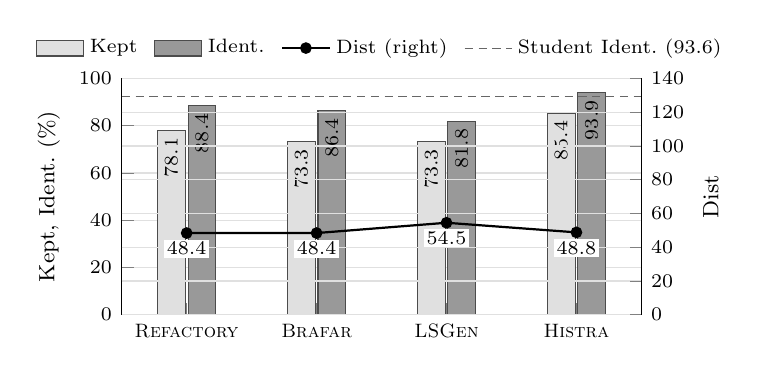
\begin{tikzpicture}
\begin{axis}[close, axis y line*=left, ylabel={Kept, Ident.\ (\%)},
  legend style={at={(0.5,1.04)}, anchor=south, legend columns=-1, draw=none, font=\scriptsize, /tikz/every even column/.append style={column sep=4pt}}]
% rows:figclosebar
\addplot[close kept] coordinates {(0,78.1) (1,73.3) (2,73.3) (3,85.4)};
\addplot[close ident] coordinates {(0,88.4) (1,86.4) (2,81.8) (3,93.9)};
\addplot[close stu] coordinates {(-0.5,92.4) (3.5,92.4)};
% end rows
\addlegendentry{Kept} \addlegendentry{Ident.}
\addlegendimage{sharp plot, black, thick, mark=*, mark size=1.7pt}\addlegendentry{Dist (right)}
\addlegendimage{sharp plot, densely dashed, black!60}\addlegendentry{Student Ident.\ (93.6)}
\end{axis}
\begin{axis}[close, axis y line*=right, axis x line=none, ymax=140, ytick={0,20,...,140}, ylabel={Dist}]
% rows:figclosedist
\addplot[close dist] coordinates {(0,48.4) (1,48.4) (2,54.5) (3,48.8)};
% end rows
\end{axis}
\end{tikzpicture}
\caption{Closeness of passing patches to the students' own fixes on the trajectories fixed by all techniques}
\label{fig:rq-close}
\end{figure}

% Figure~\ref{fig:rq-close}는 모든 기법이 고친 trajectory에서 각 기법의 Kept와 Ident(막대, 왼쪽 축), Dist(선, 오른쪽 축)를 보여 주며, 점선은 학생 자신의 수정의 Ident를 나타낸다. Kept에서 \textsc{Histra}는 학생들이 자신의 수정에서 유지한 코드의 85.4\%를 유지하여 \textsc{Refactory}(78.1\%), \textsc{Brafar}(73.3\%), \textsc{LSGen}(73.3\%)보다 각각 9.4\%, 16.6\%, 16.6\% 많았다. Ident에서 \textsc{Histra}는 학생 식별자의 93.9\%를 유지하여 각각 6.2\%, 8.7\%, 14.8\% 많았고, 학생 자신의 수정(92.4\%)과 비슷하였다. Dist에서 \textsc{Histra}의 패치와 $P_{\mathit{ac}}$ 사이의 거리는 48.8로, \textsc{Refactory}와 \textsc{Brafar}(48.4)와 비슷하고 \textsc{LSGen}(54.5)보다 10.4\% 작았다. 종합하면, \textsc{Histra}는 학생들이 자신의 수정에서 유지한 코드와 식별자를 가장 많이 유지하였다.
Figure~\ref{fig:rq-close} shows Kept and Ident (bars, left axis) and Dist (line, right axis) of each technique on the trajectories that all techniques fixed; the dashed line marks the Ident of the students' own fixes. In terms of Kept, \textsc{Histra} kept 85.4\% of the code that the students kept in their own fixes, a relative increase of 9.4\%, 16.6\%, and 16.6\% over \textsc{Refactory} (78.1\%), \textsc{Brafar} (73.3\%), and \textsc{LSGen} (73.3\%), respectively. In terms of Ident, \textsc{Histra} kept 93.9\% of the student's identifiers, a relative increase of 6.2\%, 8.7\%, and 14.8\% over them, respectively, similar to the students' own fixes (92.4\%). In terms of Dist, the distance between the patches of \textsc{Histra} and $P_{\mathit{ac}}$ was 48.8, similar to that of \textsc{Refactory} and \textsc{Brafar} (48.4) and 10.4\% smaller than that of \textsc{LSGen} (54.5). Overall, \textsc{Histra} kept the most of the code and identifiers that the students kept in their own fixes.

% \textsc{Histra}의 패치가 학생의 코드를 더 유지한 데에는 두 가지 이유가 있다. 첫째, $\mathsf{Merge}$는 참조 프로그램의 변수를 학생의 이름으로 바꾸고 학생의 식별자를 유지하므로(Section~\ref{sec:repair}), fallback 패치도 학생 식별자의 91.0\%를 유지한 반면, 프로그램 전체를 새로 생성하는 \textsc{LSGen}은 18.2\%를 바꾸었다. 둘째, Kept와 Dist의 이점은 이력이 학생이 고친 곳을 가리킨 trajectory에서 나왔다. 학생 자신의 수정이 skeleton을 바꾸지 않은 391개 trajectory에서 \textsc{Histra}는 학생이 유지한 코드를 baseline들보다 10.8--19.3\% 더 유지하였고, $P_{\mathit{ac}}$와의 거리도 3.5--18.1\% 작았다. 반면 학생이 skeleton도 바꾼 267개 trajectory에서는 \textsc{Histra}가 학생이 바꾼 skeleton 코드까지 유지하려 하여 거리가 0.9--8.4\% 컸지만, 여전히 학생이 유지한 코드를 가장 많이 유지하였다. 이러한 결과는 학생 자신의 이력이 학생이 실제로 고치는 곳을 가리킴을 보여 준다.
Two reasons explain why the patches of \textsc{Histra} kept more of the student's code. First, $\mathsf{Merge}$ renames the variables of the reference program to the student's and keeps the student's identifiers (Section~\ref{sec:repair}), so even the fallback patches kept 91.0\% of the student's identifiers, whereas \textsc{LSGen}, which generates the whole program anew, changed 18.2\% of them. Second, the advantages in Kept and Dist came from the trajectories in which the history pointed to where the student fixed. On the 391 trajectories in which the student's own fix left the skeleton unchanged, \textsc{Histra} kept 10.8--19.3\% more of the code that the student kept than the baselines, and its distance to $P_{\mathit{ac}}$ was 3.5--18.1\% smaller. On the 267 trajectories in which the student also changed the skeleton, \textsc{Histra} tried to keep the skeleton code that the student changed, so its distance was 0.9--8.4\% larger, but it still kept the most of the code that the student kept. These results show that the student's own history points to where the student actually fixes.

\subsection{RQ3: Ablation Study}\label{sec:rq2}

% RQ3는 학생의 이력과 \textsc{Histra}의 각 설계 선택이 효과에 얼마나 기여하는지 확인한다. 이를 위해 \textsc{Histra}를 다섯 변형 및 네 대조군과 비교하였다. 각 변형은 Algorithm~\ref{alg:histra}의 설계 선택 하나를 빼거나 바꾼다. \textsc{Histra}$-$Norm은 정규화 없이 원래의 syntax tree를 스케치하고(2번째 줄), \textsc{Histra}$-$Hole은 hole-only phase를 생략하며(7번째 줄의 $m = \mathit{hole}$), \textsc{Histra}$-$Kept는 후보를 phase, 순서 모드, 검색 순위로만 정렬하고(10번째 줄), \textsc{Histra}$-$Min은 처음 통과한 후보를 최소화 없이 반환하며(12번째 줄), \textsc{Histra}$_{\mathit{size}}$는 $\mathsf{Minimize}$의 되돌리기를 skeleton과 무관하게 subtree 크기로만 정렬한다(12번째 줄). 대조군은 이력으로 얻은 hole을 없애거나 다른 hole로 바꾼다. \textsc{Histra}$_{\emptyset}$는 $H = \emptyset$으로 실행하여 이력을 무시한다는 점만 \textsc{Histra}와 다르다. \textsc{Histra}$_{\mathit{rand}}$는 이력으로 얻은 hole을 같은 수의, 같은 종류이고 크기가 가장 가까운 무작위 subtree로 바꾼다(세 번 뽑은 평균). \textsc{Histra}$_{\mathit{frac}}$는 이력을 무시하고, 이력으로 얻은 hole이 벤치마크 전체에서 덮는 비율인 48.5\%만큼 모든 프로그램의 문장 및 식 노드를 무작위 subtree로 hole로 바꾼다. \textsc{Histra}$_{\mathit{FL}}$은 이력을 무시하고 spectrum 기반 Fault Localization(FL)으로 hole을 얻는다. 즉, 테스트에 대한 $b$의 line coverage에서 Ochiai 점수~\cite{abreu2006evaluation}가 가장 높은 문장을 hole로 바꾼다.
RQ3 examines how much the student's history and each design choice of \textsc{Histra} contribute to its effectiveness. To this end, we compared \textsc{Histra} with five variants and four controls. Each variant removes or replaces one design choice of Algorithm~\ref{alg:histra}: \textsc{Histra}$-$Norm sketches the raw syntax trees without normalization (line~2); \textsc{Histra}$-$Hole skips the hole-only phase ($m = \mathit{hole}$ at line~7); \textsc{Histra}$-$Kept orders the candidates by their phase, order mode, and the rank of their retrieved programs only (line~10); \textsc{Histra}$-$Min returns the first passing candidate without minimization (line~12); and \textsc{Histra}$_{\mathit{size}}$ orders the reverts of $\mathsf{Minimize}$ by subtree size alone, without regard to the skeleton (line~12). Each control removes the history-derived holes or replaces them with other holes. \textsc{Histra}$_{\emptyset}$ is \textsc{Histra} run with $H = \emptyset$ and thus differs from it only in ignoring the history. \textsc{Histra}$_{\mathit{rand}}$ replaces the history-derived holes with as many random subtrees of the same kinds and the closest sizes (averaged over three draws). \textsc{Histra}$_{\mathit{frac}}$ ignores the history and turns into holes random subtrees that cover 48.5\% of the statement and expression nodes of every program, the share that the history-derived holes cover across the benchmark. \textsc{Histra}$_{\mathit{FL}}$ ignores the history and obtains its holes from spectrum-based Fault Localization (FL): it turns into holes the statements with the highest Ochiai score~\cite{abreu2006evaluation} over the line coverage of $b$ on the tests.

\begin{table}[h]
\caption{Ablation of \textsc{Histra} (\%), with the relative change from \textsc{Histra} in parentheses}
\label{tab:ablation}
\centering
\footnotesize
\begin{tabular}{l|r|r|r}
\toprule
\textbf{Configuration} & \textbf{Fixed} & \textbf{Skeleton loss} & \textbf{Intact patches} \\
\midrule\midrule
% rows:rq2
\textsc{Histra} & 96.5 & 18.7 & 42.6 \\
\midrule
\multicolumn{4}{l}{\textit{Design choice removed or replaced}} \\
\textsc{Histra}$-$Hole & 96.1 & 21.8 ($+$16.6\%) & 31.8 ($-$25.5\%) \\
\textsc{Histra}$-$Kept & 96.5 & 20.3 ($+$8.2\%) & 41.1 ($-$3.6\%) \\
\textsc{Histra}$-$Min & 96.5 & 19.8 ($+$5.5\%) & 40.1 ($-$6.0\%) \\
\textsc{Histra}$-$Norm & 96.4 & 18.8 ($+$0.4\%) & 42.5 ($-$0.4\%) \\
\textsc{Histra}$_{\mathit{size}}$ & 96.5 & 18.7 (0.0\%) & 42.6 ($-$0.1\%) \\
\midrule
\multicolumn{4}{l}{\textit{Source of holes}} \\
\textsc{Histra}$_{\emptyset}$ & 96.1 & 24.7 ($+$32.1\%) & 29.2 ($-$31.5\%) \\
\textsc{Histra}$_{\mathit{frac}}$ & 96.2 & 23.7 ($+$26.5\%) & 30.1 ($-$29.5\%) \\
\textsc{Histra}$_{\mathit{FL}}$ & 96.2 & 20.9 ($+$11.6\%) & 37.4 ($-$12.4\%) \\
\textsc{Histra}$_{\mathit{rand}}$ & 96.2 & 19.5 ($+$4.1\%) & 40.6 ($-$4.8\%) \\
% end rows
\bottomrule
\end{tabular}
\end{table}

% Table~\ref{tab:ablation}은 \textsc{Histra}와 각 변형 및 대조군의 repair rate(Fixed), skeleton loss, intact patch 비율을 보여 주며, 괄호 안은 \textsc{Histra} 대비 상대 변화이다. 모든 구성의 repair rate는 96.1--96.5\%로 비슷하므로, 차이는 패치가 skeleton을 얼마나 지키는지에서 나타났다. 먼저 설계 선택 중에서는 hole-only phase의 기여가 가장 컸다. 이를 생략한 \textsc{Histra}$-$Hole은 skeleton loss가 16.6\% 늘고 intact patch가 25.5\% 줄어, intact patch 비율(31.8\%)이 \textsc{Histra}$_{\emptyset}$(29.2\%)에 가까워졌다. 즉, 이력은 주로 hole-only phase를 통해 패치에 반영된다. 후보를 $\mathsf{Kept}$로 정렬하지 않거나(\textsc{Histra}$-$Kept) 통과 패치를 최소화하지 않으면(\textsc{Histra}$-$Min) skeleton loss가 각각 8.2\%와 5.5\% 늘었다. 반면 되돌리기를 영역 대신 크기로만 정렬하거나(\textsc{Histra}$_{\mathit{size}}$) 정규화를 생략해도(\textsc{Histra}$-$Norm) 차이는 거의 없었다. 검증 예산 안에서는 두 순서가 대개 같은 패치에 이르고, 학생들이 연속된 제출 사이에 동등한 형태를 바꿔 쓰는 일이 드물어 정규화가 skeleton을 바꾼 trajectory가 14.8\%뿐이었기 때문이다. 종합하면, \textsc{Histra}의 효과는 hole과 그 hole 안을 먼저 고치는 hole-only phase에서 대부분 나오며, Kept 정렬과 최소화가 이를 보완한다.
Table~\ref{tab:ablation} shows the repair rate (Fixed), skeleton loss, and share of intact patches of \textsc{Histra} and each variant and control, with the relative change from \textsc{Histra} in parentheses. Since all configurations repaired 96.1 to 96.5\% of the submissions, the differences appeared in how much of the skeleton the patches kept. First, among the design choices, the hole-only phase contributed the most. Skipping it (\textsc{Histra}$-$Hole) increased the skeleton loss by 16.6\% and decreased intact patches by 25.5\%, bringing their share (31.8\%) close to that of \textsc{Histra}$_{\emptyset}$ (29.2\%); that is, the history takes effect mainly through the hole-only phase. Not ordering the candidates by $\mathsf{Kept}$ (\textsc{Histra}$-$Kept) or not minimizing the passing patch (\textsc{Histra}$-$Min) increased the skeleton loss by 8.2\% and 5.5\%, respectively. In contrast, ordering the reverts by size instead of region (\textsc{Histra}$_{\mathit{size}}$) or skipping normalization (\textsc{Histra}$-$Norm) made almost no difference: within the validation budget, both orders mostly reach the same patch, and because students rarely switch between equivalent forms across consecutive submissions, normalization changed the skeleton of only 14.8\% of the trajectories. Overall, the effect of \textsc{Histra} comes mostly from the holes and from the hole-only phase that repairs inside them first, complemented by the $\mathsf{Kept}$ ordering and minimization.

% hole의 출처를 바꾸면 이력의 기여가 더 크게 드러났다. 이력을 무시한 \textsc{Histra}$_{\emptyset}$는 skeleton loss가 32.1\% 늘고 intact patch가 31.5\% 줄었다. 이력 없이 hole이 덮는 비율만 맞춘 \textsc{Histra}$_{\mathit{frac}}$도 skeleton loss가 26.5\% 늘고 intact patch가 29.5\% 줄어 \textsc{Histra}$_{\emptyset}$와 비슷하였다. 반면 이력이 정한 hole의 수, 종류, 크기는 그대로 두고 위치만 무작위로 바꾼 \textsc{Histra}$_{\mathit{rand}}$는 skeleton loss가 4.1\%만 늘고 intact patch가 4.8\%만 줄었으며, 이 차이는 세 번의 무작위 추출 모두에서 나타났다. 즉, 이력은 무엇보다 각 프로그램에 hole이 얼마나, 어떤 크기로 필요한지를 정함으로써 기여한다. 같은 비율의 hole이라도 학생이 계속 고쳐 온 양에 맞추지 않으면 효과가 사라지며, hole의 위치를 이력으로 정하는 것은 그 위에 작지만 일관된 이득을 더한다. FL로 hole을 얻은 \textsc{Histra}$_{\mathit{FL}}$은 skeleton loss가 11.6\% 늘고 intact patch가 12.4\% 줄었다. FL은 문장을 그것을 실행하는 테스트로만 구별하므로, 모든 테스트가 모든 문장을 실행하는 짧은 프로그램에서는 프로그램 전체를 hole로 만들었기 때문이다(trajectory의 12.5\%, 이력은 3.0\%). 종합하면, 학생의 이력으로 정한 intent skeleton은 FL로 정한 hole보다 학생의 의도를 더 잘 보존하며, \textsc{Histra}의 효과 대부분은 이력이 각 프로그램에서 수정할 양을 정하는 데서 나온다.
Changing the source of the holes revealed the contribution of the history even more clearly. Ignoring the history (\textsc{Histra}$_{\emptyset}$) increased the skeleton loss by 32.1\% and decreased the share of intact patches by 31.5\%. Holes that only match the share that the history-derived holes cover (\textsc{Histra}$_{\mathit{frac}}$) behaved similarly, increasing the skeleton loss by 26.5\% and decreasing intact patches by 29.5\%. In contrast, keeping the number, kinds, and sizes of the history-derived holes and randomizing only their locations (\textsc{Histra}$_{\mathit{rand}}$) increased the skeleton loss by only 4.1\% and decreased intact patches by only 4.8\%, consistently across the three draws. The history thus contributes mainly by deciding how many holes of which sizes each program needs: holes that cover the same share lose their effect unless they match how much the student kept revising, and placing them where the history indicates adds a small but consistent gain on top. Holes from FL (\textsc{Histra}$_{\mathit{FL}}$) increased the skeleton loss by 11.6\% and decreased intact patches by 12.4\%: FL tells statements apart only by the tests that execute them, so in short programs, where every test executes every statement, it turned the whole program into holes (12.5\% of the trajectories, compared with 3.0\% for the history). Overall, the intent skeleton derived from the student's own history preserves the student's intent better than holes from FL, and most of the effect of \textsc{Histra} comes from the history deciding how much of each program to open for repair.

\subsection{RQ4: Instructors' Choice of Feedback}\label{sec:rq-expert}

% RQ4는 skeleton을 더 많이 유지하는 패치가 강사가 보기에도 더 나은 피드백인지 확인한다. 이를 위해 저자가 아닌 외부 강사 2명이 패치 쌍을 블라인드로 평가하였다. 두 강사는 대학에서 3년 이상 강의하였고, 현재 신입생 대상 과목(문제해결과 컴퓨팅 사고, 프로그래밍 기초와 실습)을 가르친다. 이력의 효과만 분리하도록, 이력을 무시한다는 점만 다른 \textsc{Histra}$_{\emptyset}$의 패치와 비교하였다. 두 패치는 같은 파이프라인의 출력이고 모든 프로그램을 같은 형식으로 정리하여 보여 주므로, 강사는 패치의 출처를 알 수 없다. 두 기법이 모두 고치고 skeleton이 비어 있지 않으며 두 패치가 다른 trajectory에서, 어느 문제에도 치우치지 않도록 고정 seed로 문제마다 7쌍씩 모두 98쌍을 추출하였다. 각 항목은 문제 설명, 학생의 버기 제출 $b$, 그리고 $b$에 대한 두 패치의 diff를 무작위 순서로 보여 준다. 강사는 먼저 이 정보만으로 이 학생에게 피드백으로 보여 줄 패치를 고르고(P-Feedback), 이어서 나타나는 학생의 이전 제출을 본 뒤 학생이 하려던 바를 더 잘 살린 패치를 골랐다(P-Intent). 즉, P-Feedback은 강사가 제출 하나만 볼 때와 같은 정보로 판단하고, P-Intent는 \textsc{Histra}와 같은 이력으로 판단하되 skeleton은 보여 주지 않으므로 강사가 의도를 스스로 읽는다. 두 질문 모두 두 패치가 비슷하다고 답할 수도 있었다. 일치도는 불일치를 조정하기 전의 linear weighted Cohen's $\kappa$로 보고하고, 선호는 exact sign test로 검정하였다.
RQ4 examines whether patches that keep more of the skeleton are also better feedback in the eyes of instructors. To this end, two external instructors, neither of whom is an author, rated pairs of patches in a blinded study. Both have taught at a university for at least three years and currently teach first-year courses (problem solving and computational thinking, and programming fundamentals). To isolate the effect of the history, we compared the patches of \textsc{Histra} with those of \textsc{Histra}$_{\emptyset}$, which differs only in ignoring the history; since both come from the same pipeline and all programs were shown in the same normalized format, the instructors could not tell the source of a patch. From the trajectories that both techniques fix, whose skeleton is non-empty, and whose two patches differ, we sampled seven pairs per problem (98 pairs) with a fixed seed, so that no problem dominates the sample. Each item showed the problem statement, the student's buggy submission $b$, and the diffs of the two patches against $b$ in random order. From this information alone, the instructors first chose the patch they would rather show this student as feedback (P-Feedback). The student's earlier submissions then appeared, and the instructors chose the patch that better preserves what the student was trying to do (P-Intent). P-Feedback thus rests on what an instructor sees for a single submission, whereas P-Intent rests on the same history as \textsc{Histra} but never on the skeleton, so the instructors read the intent on their own. For both questions, the instructors could also answer that the two patches are about the same. We report the agreement as the linear weighted Cohen's $\kappa$ before resolving disagreements and test the preferences with exact sign tests.

% 조정을 거친 판정에서, 먼저 P-Feedback에서 강사들은 전체 98쌍의 77.6\%에서 \textsc{Histra}의 패치를 피드백으로 골랐으며, 강사별로도 73.5\%와 83.7\%로 \textsc{Histra}를 선호하였다. P-Intent에서도 강사들은 78.6\%의 쌍에서 \textsc{Histra}의 패치가 학생의 의도를 더 잘 살렸다고 판단하였다(강사별 75.5\%와 83.7\%). 두 질문 모두 선호는 유의하였고(exact sign test, $p < 0.001$), 두 패치가 비슷하다는 응답은 없었다. 조정 전 두 강사의 일치도는 P-Feedback에서 linear weighted $\kappa = 0.70$(일치율 90\%), P-Intent에서 0.75(92\%)였다. 종합하면, 강사들은 이력 없이 같은 파이프라인으로 만든 패치보다 \textsc{Histra}의 패치를 피드백으로 선호하였다.
After adjudication, for P-Feedback, the instructors chose the patch of \textsc{Histra} as feedback in 77.6\% of the 98 pairs, and each instructor preferred it as well (73.5\% and 83.7\%). For P-Intent, they judged the patch of \textsc{Histra} to better preserve the student's intent in 78.6\% of the pairs (75.5\% and 83.7\% for the two instructors). Both preferences were significant (exact sign test, $p < 0.001$), and neither instructor answered that the two patches are about the same. Before adjudication, the instructors agreed with a linear weighted $\kappa$ of 0.70 for P-Feedback (90\% raw agreement) and 0.75 for P-Intent (92\%). Overall, the instructors preferred the patches of \textsc{Histra} as feedback to those of the same pipeline without the history.

\begin{figure}[h]
\centering
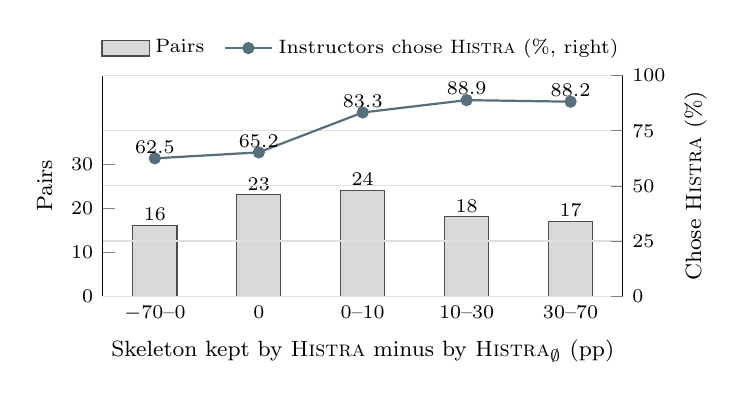
\begin{tikzpicture}
\begin{axis}[expg, axis y line*=left, axis x line*=bottom, ymin=0, ymax=50, ytick={0,10,20,30}, ylabel={Pairs},
  xlabel={Skeleton kept by \textsc{Histra} minus by \textsc{Histra}$_{\emptyset}$ (pp)},
  legend style={at={(0.5,1.03)}, anchor=south, legend columns=-1, draw=none, font=\scriptsize, /tikz/every even column/.append style={column sep=5pt}}]
% rows:figexpcount
\addplot[exp count] coordinates {(0,16) (1,23) (2,24) (3,18) (4,17)};
% end rows
\addlegendentry{Pairs}
\addlegendimage{exp rate}\addlegendentry{Instructors chose \textsc{Histra} (\%, right)}
\end{axis}
\begin{axis}[expg, axis y line*=right, axis x line=none, ymin=0, ymax=100, ytick={0,25,50,75,100}, ymajorgrids, grid style={black!12}, ylabel={Chose \textsc{Histra} (\%)}]
% rows:figexprate
\addplot[exp rate] coordinates {(0,62.5) (1,65.2) (2,83.3) (3,88.9) (4,88.2)};
% end rows
\end{axis}
\end{tikzpicture}
\caption{Rated pairs by how much more of the skeleton the patch of \textsc{Histra} keeps than that of \textsc{Histra}$_{\emptyset}$, and the share of them in which the instructors chose the patch of \textsc{Histra} as feedback}
\label{fig:expert}
\end{figure}

% 강사들이 \textsc{Histra}의 패치를 선호한 것은 그 패치가 학생의 의도를 살렸기 때문이다. 이력을 보기 전에 피드백으로 고른 패치는 98쌍 중 97쌍에서, 이력을 본 뒤 학생의 의도를 더 잘 살렸다고 판단한 패치와 같았다. Figure~\ref{fig:expert}는 평가한 쌍을 \textsc{Histra}의 패치가 \textsc{Histra}$_{\emptyset}$의 패치보다 skeleton을 얼마나 더 유지했는지에 따라 나누고, 구간별 쌍의 수(막대)와 강사들이 \textsc{Histra}를 피드백으로 고른 비율(꺾은선)을 보여 준다. \textsc{Histra}가 skeleton을 더 유지한 쌍은 59쌍으로 덜 유지한 쌍(16쌍)의 3.7배였으며, 강사들이 \textsc{Histra}를 고른 비율은 \textsc{Histra}가 덜 유지하거나 같은 양을 유지한 쌍에서 62.5\%와 65.2\%였지만 더 유지한 쌍에서는 83.3--88.9\%로 높아졌다. P-Intent도 같은 경향을 보였다. 이러한 결과는 강사들이 학생이 유지해 온 코드를 지키는 패치를 피드백으로 고르며, \textsc{Histra}가 이력으로 지키는 intent skeleton이 바로 그 코드임을 보여 준다.
The instructors preferred the patches of \textsc{Histra} because those patches preserved the student's intent. In 97 of the 98 pairs, the patch chosen as feedback before seeing the history was the one judged to better preserve the student's intent after seeing it. Figure~\ref{fig:expert} divides the rated pairs by how much more of the skeleton the patch of \textsc{Histra} kept than that of \textsc{Histra}$_{\emptyset}$, and shows the number of pairs in each range (bars) and the share of them in which the instructors chose the patch of \textsc{Histra} as feedback (line). The patch of \textsc{Histra} kept more of the skeleton in 59 pairs, 3.7 times as many as the 16 pairs in which it kept less, and the share in which the instructors chose it rose from 62.5\% and 65.2\% in the pairs in which it kept less or the same amount to 83.3--88.9\% in the pairs in which it kept more; P-Intent followed the same trend. These results show that instructors choose as feedback the patches that keep the code that the student has kept, and that the intent skeleton, which \textsc{Histra} keeps by using the history, is exactly that code.

\subsection{Discussion}\label{sec:discussion}

% \textbf{강사를 위한 시사점.} 우리의 결과는 이력 기반 패치를 피드백으로 쓰는 세 가지 방법을 시사한다. 첫째, hole은 학생 자신의 수정이 바꾼 코드의 64.4\%를 포함하므로(Section~\ref{sec:prelim-limit}), hole을 강조하는 것만으로도 학생에게 살펴볼 곳을 알려 줄 수 있다. 둘째, fallback 패치는 hole-only 패치보다 학생의 코드를 더 많이 다시 쓰므로(Section~\ref{sec:rq1}), 그대로 보여 주기보다 힌트로 바꾸어 주는 것이 낫다. 셋째, 여러 패치가 테스트를 통과할 때는 skeleton을 더 많이 유지하는 패치를 보여 주는 것이 좋다. 강사들의 선호는 패치가 skeleton을 더 유지할수록 뚜렷하였다(Section~\ref{sec:rq-expert}).
\textbf{Implications for instructors.} Our results suggest three ways to use history-guided patches as feedback. First, the holes contain 64.4\% of the code that the student's own fix changes (Section~\ref{sec:prelim-limit}), so highlighting them already points the student to where to look. Second, the fallback patches rewrite more of the student's code than the hole-only patches (Section~\ref{sec:rq1}) and are thus better turned into hints than shown as is. Third, when several patches pass the tests, a tool should show the one that keeps more of the skeleton: the instructors' preference grew with how much of the skeleton a patch kept (Section~\ref{sec:rq-expert}).

% \textbf{패치의 전달.} 패치는 그대로 보여 줄 수도 있고, hole 안의 변경만 남기거나, 힌트를 생성하는 LLM의 입력으로 줄 수도 있다~\cite{phung2024automating}. 모델에 해답을 주면 힌트가 그 해답 쪽으로 치우치므로~\cite{roest2024next}, 학생의 접근을 보존하는 패치가 이런 입력으로도 더 적합할 것이다. 자동 생성된 수정은 초보 학생보다 조교에게 더 도움이 되었다는 보고~\cite{yi2017feasibility}를 고려하면, 조교를 통한 전달도 현실적인 선택지이다. 어떤 전달 방식이 학습에 가장 도움이 되는지는 학생 대상 연구로 확인할 과제로 남긴다.
\textbf{Delivering patches.} A patch can be shown as is, reduced to the changes inside the holes, or given as input to an LLM that generates hints~\cite{phung2024automating}. Since giving a model a solution steers its hints toward that solution~\cite{roest2024next}, a patch that preserves the student's approach is likely a better input for such hints as well. Since generated repairs were found to help teaching assistants more than novices~\cite{yi2017feasibility}, delivery through teaching assistants is another realistic option. Which form of delivery helps learning most remains to be studied with students.

\subsection{Threats to Validity}\label{sec:threats}

% 우리의 벤치마크는 AtCoder 14문제에 대한 참가자의 Python 제출로 이루어져, 강의 과제나 다른 언어를 대표하지 않을 수 있다. 다만 문제들은 입문 프로그래밍의 개념을 다루며(Table~\ref{tab:bench}), Python을 택한 것은 모든 baseline의 공개 구현이 Python을 대상으로 하기 때문이다. 또한 \textsc{Histra}의 Sketch와 Merge는 AST와 tree edit mapping만 쓰므로, 다른 언어에는 그 언어의 파서와 정규화 규칙만 있으면 옮길 수 있다. 벤치마크는 정답 전에 두 번 이상 틀린 trajectory만 포함하는데, 한 번만 틀린 학생에게는 이력이 없어 intent skeleton을 정의할 수 없기 때문이다. 이런 학생에게 \textsc{Histra}는 이력 없이 실행되며, 이는 RQ3의 \textsc{Histra}$_{\emptyset}$와 같은 설정이다. 이 설정에서도 \textsc{Histra}는 모든 baseline보다 많은 버기 제출을 고쳤다(Section~\ref{sec:rq2}). 또한 이력이 이전 제출 하나뿐인, 즉 벤치마크에서 가장 짧은 이력을 가진 trajectory(34.3\%)에서도 \textsc{Histra}는 모든 baseline보다 skeleton을 잘 지켰다.
Our benchmark consists of the Python submissions of contestants to 14 AtCoder problems and may not represent course assignments or other languages. However, the problems exercise concepts of introductory programming (Table~\ref{tab:bench}), and we chose Python because the released implementations of all baselines target Python. Moreover, the Sketch and Merge of \textsc{Histra} use only ASTs and tree edit mappings, so porting \textsc{Histra} to another language requires only a parser and normalization rules for that language. The benchmark includes only trajectories with at least two wrong-answer submissions, because a student who failed only once has no history from which to derive an intent skeleton. For such a student, \textsc{Histra} runs without the history, which is the setting of \textsc{Histra}$_{\emptyset}$ in RQ3; even in this setting, \textsc{Histra} fixed more buggy submissions than every baseline (Section~\ref{sec:rq2}). Moreover, on the trajectories whose history has only one earlier submission, i.e., the shortest history in our benchmark (34.3\% of the trajectories), \textsc{Histra} kept more of the skeleton than every baseline.

\section{Related Work}\label{sec:related}

% TODO(MENTORED): once MENTORED's run is in, add it to the baselines or give its exclusion reason here (and in Baselines).
% \textbf{APR for Programming Assignments.} Section~\ref{sec:prelim-repair}에서 설명한 기법들 외에도 많은 기법이 학생 제출을 자동으로 수정한다. alignment-based 기법 중 \textsc{Verifix}~\cite{ahmed2022verifix}는 강사의 참조 해답과 정렬하여 검증된 수정을 만들고, Kaleeswaran et al.~\cite{kaleeswaran2016semi}은 강사의 피드백을 제출 군집 안에 전파하고, Song et al.~\cite{song2021context}은 변수가 쓰이는 맥락으로 프로그램을 정렬한다. localization-based 기법으로는 버그가 있는 줄(의 일부)을 가리고 모델이 채우게 하는 infilling 기반 수정이 일반적인 APR~\cite{xia2022less}과 학생 프로그램~\cite{koutcheme2023automated}에 적용되었다. knowledge-based 기법 중 \textsc{Referent}~\cite{heo2023referent}는 과제 정보를 이용하는 Transformer 모델로 정답 제출 없이도 수정을 생성하고, 다른 기법들은 신경망 모델이나 LLM으로 프로그램을 고친다~\cite{pu2016sk_p, liu2024fastfixer, yang2024cref}. LLM 기반 기법은 맞는 참조 프로그램이 필요 없지만 필요 이상으로 다시 쓰는 경향이 있으며~\cite{orvalho2025counterexample, dai2025less, phung2023generative}, 참조 프로그램을 함께 주면 그 참조 프로그램을 그대로 돌려주기도 한다~\cite{xie2024brafar}. 우리는 세 계열에서 각각 \textsc{Refactory}, \textsc{Brafar}, \textsc{LSGen}을 baseline으로 삼았다. \textsc{Clara}는 \textsc{Refactory}보다~\cite{hu2019re}, \textsc{AdaPatcher}, \textsc{PyDex}, \textsc{PaR}은 \textsc{LSGen}보다~\cite{dai2026learner} 적게 고쳤고, \textsc{Sarfgen}과 \textsc{Qlose}는 구현이 공개되지 않았으며, \textsc{Verifix}와 \textsc{Cegis}는 C 프로그램만 다루고, \textsc{AutoGrader}는 강사가 작성한 오류 모델이 필요하며, \textsc{Refazer}는 벤치마크의 파서를 지원하지 않아 제외하였다. 대신 RQ3에서 FL로 얻은 hole을 이력에서 얻은 hole과 비교하였다(Section~\ref{sec:rq2}).
\textbf{APR for Programming Assignments.} Beyond the techniques described in Section~\ref{sec:prelim-repair}, many techniques automatically repair student submissions. Among alignment-based techniques, \textsc{Verifix}~\cite{ahmed2022verifix} aligns the submission with an instructor's reference solution to produce verified repairs, Kaleeswaran et al.~\cite{kaleeswaran2016semi} propagate an instructor's feedback within clusters of submissions, and Song et al.~\cite{song2021context} align programs by the contexts in which their variables are used. As a localization-based technique, infilling-based repair, which masks (parts of) buggy lines and lets a model fill them, has been applied to general APR~\cite{xia2022less} and to student programs~\cite{koutcheme2023automated}. Among knowledge-based techniques, \textsc{Referent}~\cite{heo2023referent} generates repairs even without correct submissions using a Transformer model that exploits assignment information, and others repair programs with neural models or LLMs~\cite{pu2016sk_p, liu2024fastfixer, yang2024cref}. LLM-based techniques need no matching reference program but tend to rewrite more than needed~\cite{orvalho2025counterexample, dai2025less, phung2023generative}, and given a reference program, an LLM may return that program verbatim~\cite{xie2024brafar}. We selected \textsc{Refactory}, \textsc{Brafar}, and \textsc{LSGen} as baselines from the three groups, respectively. We excluded \textsc{Clara}, which repaired fewer submissions than \textsc{Refactory}~\cite{hu2019re}; \textsc{AdaPatcher}, \textsc{PyDex}, and \textsc{PaR}, which repaired fewer than \textsc{LSGen}~\cite{dai2026learner}; \textsc{Sarfgen} and \textsc{Qlose}, whose implementations are not publicly available; \textsc{Verifix} and \textsc{Cegis}, which handle only C programs; \textsc{AutoGrader}, which requires an instructor-written error model; and \textsc{Refazer}, whose parser does not support our benchmark. RQ3 instead compares holes from FL with those from the history (Section~\ref{sec:rq2}).

% \textbf{Feedback on the Student's Own Work.} 우리의 연구는 제출 이력에서 배우거나 학생의 프로그램에 맞춘 피드백을 주는 기법들과 관련된다. Hint Factory와 ITAP 같은 힌트 생성기는 많은 학생이 정답에 이르기까지 거친 경로를 수집하고~\cite{barnes2008toward, paassen2018continuous, rivers2017data}, knowledge-based 수정 기법은 다른 학생들의 버기 제출에서 고친 제출로의 편집에서 배우며~\cite{rolim2017learning, zhang2024pydex, liu2024fastfixer, dai2026learner}, 일반적인 APR은 여러 프로젝트의 과거 수정~\cite{le2016history}이나 HAFix처럼 버그가 있는 줄의 이력~\cite{shi2026hafix}을 맥락으로 쓴다. 학생 자신의 직전 제출을 보는 도구도 있지만, 힌트를 어떻게 이어 갈지 정하는 데에만 쓴다~\cite{paiva2025incremental}. 수정을 피드백으로 쓰는 것의 교육적 효과도 연구되었다. 수정 피드백은 학생들이 사람 튜터의 피드백보다 컴파일 오류를 빨리 해결하게 했지만 그 이점은 피드백이 없는 시험에서 사라졌고~\cite{ahmed2020characterizing}, 강의에 배치된 LLM 튜터의 응답은 일반적이라는 우려를 받았다~\cite{frankford2024ai}. 최근 연구는 학생의 접근을 보존하는지를 명시적인 기준으로 삼지만~\cite{koutcheme2023evaluating, koutcheme2025direct, pitts2026automated}, 그 거리 기반 목표~\cite{d2016qlose, koutcheme2025direct, dai2025less}는 프로그램의 모든 부분에 같은 비용을 매긴다. 반면 \textsc{Histra}는 도움을 받는 학생 자신의 이력을 이용해 패치가 무엇을 유지해야 할지를 결정한다. 우리가 아는 한, \textsc{Histra}는 학생 자신의 제출 이력으로부터 보존할 의도를 추론하는 첫 수정 기법이다.
\textbf{Feedback on the Student's Own Work.} Our work relates to techniques that learn from submission histories or tailor feedback to the student's program. Hint generators such as the Hint Factory and ITAP mine the paths that many students took toward a correct solution~\cite{barnes2008toward, paassen2018continuous, rivers2017data}; knowledge-based repair techniques learn from other students' edits from buggy to corrected submissions~\cite{rolim2017learning, zhang2024pydex, liu2024fastfixer, dai2026learner}; and general APR uses the past fixes of many projects~\cite{le2016history} or, as in HAFix, the history of the buggy lines~\cite{shi2026hafix} as context. A feedback tool may also look at the student's own previous submission, but only to decide how to continue its hints~\cite{paiva2025incremental}. The educational effect of repairs as feedback has also been studied: repair feedback helped students resolve compilation errors faster than feedback from human tutors, but the advantage disappeared in exams without feedback~\cite{ahmed2020characterizing}, and the responses of an LLM tutor deployed in a course raised concerns that they were generic~\cite{frankford2024ai}. Recent work makes the preservation of the student's approach an explicit criterion~\cite{koutcheme2023evaluating, koutcheme2025direct, pitts2026automated}, but its distance-based objectives~\cite{d2016qlose, koutcheme2025direct, dai2025less} charge every part of the program alike. In contrast, \textsc{Histra} uses the history of the student being helped to decide what the patch should keep. To our knowledge, \textsc{Histra} is the first repair technique that infers the intent to preserve from the student's own submission history.

\section{Conclusion}\label{sec:conclusion}

% 자동 프로그램 수정은 학생 버기 제출의 repair rate를 크게 높여 왔다. 그러나 기존 기법은 학생들이 자신의 제출에 걸쳐 유지해 온 코드인 intent skeleton의 많은 부분을 바꾼다. 본 논문은 학생 자신의 제출 이력에 드러난 의도를 보존하면서 버기 제출을 수정하는 것을 목표로 한다. 이를 위해 \textsc{Histra}는 이력에서 얻은 hole로 버기 제출을 스케치하고, 다른 학생들의 정답 프로그램을 검색하여, 먼저 hole 안에 병합한다. 실험 결과는 \textsc{Histra}가 최신 기법들보다 많은 제출을 고치면서 intent skeleton을 적게 바꾸며, 강사들이 이력 없이 얻은 패치보다 그 패치를 피드백으로 선호함을 보여 준다. 우리는 \textsc{Histra}가 학생들이 다른 사람의 해답이 아닌 자신의 시도에 대한 피드백을 받는 데 도움이 되기를 바란다.
Automated Program Repair has substantially improved the repair rate for buggy student submissions. However, existing techniques change much of the intent skeleton, the code that students kept across their own submissions. This paper aims to repair buggy submissions while preserving the intent revealed in the student's own submission history. To this end, \textsc{Histra} sketches the buggy submission with holes derived from the history, retrieves the accepted programs of other students, and merges them into the holes first. Experimental results demonstrate that \textsc{Histra} repairs more submissions than state-of-the-art techniques while changing less of the intent skeleton, and that instructors prefer its patches as feedback to those obtained without the history. We hope that \textsc{Histra} helps students receive feedback on their own attempts rather than on the solutions of others.

\section*{Data Availability}
% \textsc{Histra}, 벤치마크, 모든 실험 데이터를 \url{https://anonymous.4open.science/r/histra/}에 공개한다.
\textsc{Histra}, our benchmark, and all experimental data are available at \url{https://anonymous.4open.science/r/histra/}.

\bibliographystyle{IEEEtran}
\bibliography{references}

\end{document}
